%%%%%%%%%%%%%%%%%%%%%%%%%%%%%%%%%%%%%%%%%%%%%%%%%%%%%%%%%%%%%%%%%%%%%%%%%%%%%%%%%%%%%%%%%%%%%%%%%%%%%%%%%%%%%%%%%
\documentclass[12pt]{article}
\usepackage{latexsym,epsfig,graphicx,epstopdf,amsmath,amssymb,amscd,pifont, multirow,chicago,psfrag,paralist,dsfont,url}
\usepackage[titletoc]{appendix}
\usepackage{listings}
\usepackage{graphics}

\usepackage{subcaption}
%\usepackage[labelformat=parens,labelsep=quad,skip=3pt]{caption}
\usepackage{graphicx}
\usepackage{bm}

\usepackage{varwidth}
\usepackage{verbatim}

\newenvironment{centerverbatim}{%
  \par
  \centering
  \varwidth{\linewidth}%
  \verbatim
}{%
  \endverbatim
  \endvarwidth
  \par
}


%%%%%%%%%%%%%%%%%%%%%%%%%%%%%%%%%%%%%%%%%%%%%%%%%%%%%%%%%%%%%%%%%%%%%%%%%%%%%%%%%%%%%%%%%%%%%%%%%%%%%%%%%%%%%%%%%
\textwidth  6.6in \textheight 9.2in \topmargin -0.6in \oddsidemargin
-0.0in \evensidemargin -0.0in \pagestyle{plain}

\newcommand{\cmark}{\ding{51}}%
\newcommand{\xmark}{\ding{55}}%
\newcommand{\thetavec}{{\boldsymbol{\theta}}}
\newcommand{\veps}{\varepsilon}
\newcommand{\loglik}{\mathcal{L}}
\newcommand{\vepsvec}{{\boldsymbol{\varepsilon}}}
\newcommand{\Sigmavec}{{\boldsymbol{\Sigma}}}
\newcommand{\wvec}{{\boldsymbol{w}}}
\newcommand{\zerovec}{{\boldsymbol{0}}}
\newcommand{\onevec}{{\boldsymbol{1}}}
\newcommand{\Ivec}{{\boldsymbol{I}}}
\newcommand{\betavec}{{\boldsymbol{\beta}}}
\newcommand{\betahat}{{\widehat{\beta}}}
\newcommand{\etavec}{{\boldsymbol{\eta}}}
\newcommand{\thetavecC}{{\boldsymbol{\theta}_C}}
\newcommand{\thetavecT}{{\boldsymbol{\theta}_T}}
\newcommand{\thetaveca}{\thetavec_{1}}
\newcommand{\thetavecb}{\thetavec_{2}}
\newcommand{\EE}{\mathbb{E}}
\newcommand{\Bset}{\mathbf{B}}
\newcommand{\Xset}{\mathbf{X}}
\newcommand{\Xmat}{\mathbf{X}}
\newcommand{\Cmat}{\mathbf{C}}
\newcommand{\Zmat}{\mathbf{Z}}
\newcommand{\Pmat}{\mathbf{P}}
\newcommand{\Hmat}{\mathbf{H}}
\newcommand{\Gmat}{\mathbf{G}}
\newcommand{\pvec}{\boldsymbol{p}}
\newcommand{\Sset}{\mathbf{S}}
\newcommand{\cp}{{\textrm{CP}}}
\newcommand{\pr}{{\textrm{Pr}}}
\newcommand{\mvn}{{\textrm{MVN}}}
\newcommand{\mse}{{\textrm{MSE}}}
\newcommand{\emse}{{\textrm{EMSE}}}
\newcommand{\TAE}{{\textrm{TAE}}}
\newcommand{\MAE}{{\textrm{MAE}}}
\newcommand{\bin}{{\textrm{bin}}}
\newcommand{\enum}{{\textrm{enum}}}
\newcommand{\Var}{{\textrm{Var}}}
\newcommand{\muhat}{\widehat{\mu}}
\newcommand{\sigmahat}{\widehat{\sigma}}
\newcommand{\thetavechat}{\widehat{\thetavec}}
\newcommand{\thetavecmis}{\thetavec_{\ast}}
\newcommand{\mumis}{\mu_{\ast}}
\newcommand{\sigmamis}{\sigma_{\ast}}
\newcommand{\thetavecahat}{\widehat{\thetavec}_1}
\newcommand{\thetavecbhat}{\widehat{\thetavec}_2}
\newcommand{\amse}{{\textrm{AMSE}}}
\newcommand{\avar}{{\textrm{AVar}}}
\newcommand{\abias}{{\textrm{ABias}}}
\newcommand{\bias}{{\textrm{Bias}}}
%\newcommand{\diag}{{\textrm Diag}}
\newcommand{\Arg}{{\textrm{Arg}}}
\newcommand{\Ber}{{\textrm{Ber}}}
\newcommand{\atantwo}{{\textrm{atan2}}}
\newcommand{\ivec}{{\boldsymbol{i}}}
\newcommand{\dgoto}{\overset{d}{\rightarrow}}
\newcommand{\Pgoto}{\overset{P}{\rightarrow}}
\newcommand{\asgoto}{\overset{a.s.}{\longrightarrow}}
\newcommand{\sev}{\textrm{sev}}
\newcommand{\nor}{\textrm{nor}}
\newcommand{\N}{\textrm{N}}
\newcommand{\diag}{\textrm{Diag}}
\newcommand{\PMD}{\textrm{PMD}}
\newcommand{\wh}{\widehat}
\newcommand{\sigmaR}{\sigma_{R}}
\newcommand{\muR}{\mu_{R}}
\newtheorem{result}{Result}
\newcommand{\Xvec}{\boldsymbol{X}}
\newcommand{\Zvec}{\boldsymbol{Z}}
\newcommand{\xvec}{\boldsymbol{x}}
\newcommand{\gvec}{\boldsymbol{g}}
\newcommand{\kvec}{\boldsymbol{k}}
\newcommand{\rvec}{\boldsymbol{r}}
\newcommand{\hvec}{\boldsymbol{h}}
\newcommand{\muvec}{\boldsymbol{\mu}}
\newcommand{\minitab}[2][l]{\begin{tabular}{#1}#2\end{tabular}}
\newcommand{\fft}{\textrm{FFT}}
\newcommand{\code}{\texttt}


%mu sigma vector
\newcommand{\Sig}{\boldsymbol{\Sigma}}
\newcommand{\mvec}{\boldsymbol{\mu}}

%methods
\newcommand{\SIM}{{\textrm{SIM}}}
\newcommand{\NA}{{\textrm{NA}}}
\newcommand{\dft}{{\textrm{DFT-CF}}}



\newcommand{\qed}{\hfill\blacksquare}
\newcommand{\qedw}{\hfill \ensuremath{\Box}}


%%%%%%%%%%%%%%%%%%%%%%%%%%%%%%%%%%%%%%%%%%%%%%%%%%%%%%%%%%%%%%%%%%%%%%%%%%%%%%%%%%%%%%%%%%%%%%%%%%%%%%%%%%%%%%%%%
\def\baselinestretch{1.25}
\renewcommand{\arraystretch}{.8}
%%%%%%%%%%%%%%%%%%%%%%%%%%%%%%%%%%%%%%%%%%%%%%%%%%%%%%%%%%%%%%%%%%%%%%%%%%%%%%%%%%%%%%%%%%%%%%%%%%%%%%%%%%%%%%%%%

\usepackage[ruled,vlined]{algorithm2e}
%%%%%%%%%%%%%%%%%%%%%%%%%%%%%%%%%%%%%%%%%%%%%%%%%%%%%%%%%%%%%%%%%%%%%%%%%%%%%%%%%%%%%%%%%%%%%%%%%%%%%%%%%%%%%%%%%

%\theoremstyle{definition}
%\newtheorem{exmp}{Example}[section]



\newtheorem{example}{Example}
\newtheorem{thm}{Theorem}
\newtheorem{ppt}{Proposition}
\newtheorem{lemma}{Lemma}
\newtheorem{remark}{Remark}
\newtheorem{defn}{Definition}
\newtheorem{corl}{Corollary}

%%%%%%%%%%%%%%%%%%%%%%%%%%%%%%%%%%%%%%%%%%%%%%%%%%%%%%%%%%%%%%%%%%%%%%%%%%%%%%%%%%%%%%%%%%%%%%%%%%%%%%%%%%%%%%%%%
\def\baselinestretch{1.25}
\renewcommand{\arraystretch}{.8}
%%%%%%%%%%%%%%%%%%%%%%%%%%%%%%%%%%%%%%%%%%%%%%%%%%%%%%%%%%%%%%%%%%%%%%%%%%%%%%%%%%%%%%%%%%%%%%%%%%%%%%%%%%%%%%%%%

\setcounter{tocdepth}{2}

%-------------------------------------------------------------------------
\begin{document}
%%%%%%%%%%%%TITLE%%%%%%%%%%%%%%%%%%%%%%%%%%%%%%%%%%%

%\title{The Computing of Probability Mass Functions for the Poisson Multinomial Distribution}

\title{The Poisson Multinomial Distribution and Its Applications in Voting Theory, Ecological Inference, and Machine Learning}


%\iffalse
\author{
Zhengzhi Lin, Yueyao Wang, and Yili Hong\\[1.5ex]
{Department of Statistics, Virginia Tech, Blacksburg, VA 24061}
}
%\fi
	
\date{\today}
	
\maketitle
	%%%%%%%%%%%%%%%%%%%%%%%%%%%%%%%%%%%%%%%%%%%%%%%%%%%%%%%%%%%%%%%%%%%%%%%%%%%%%%%%%%%%%%%%%%%%%%%%%%%%%%%%%%%%%%%%
\begin{abstract}
The Poisson multinomial distribution (PMD) describes the distribution of the sum of $n$ independent-but-nonidentical random vectors, in which each random vector is of $m$ dimension, 0/1 valued, and only one of its elements can take value 1 with a certain probability. These probabilities varies from the random vectors and form an $n \times m$ matrix, which is called the success probability matrix (SPM). Each SPM uniquely defines a $\PMD$. The $\PMD$ is useful in many areas such as, voting theory, ecological inference, and machine learning. The distribution functions of $\PMD$, however, is usually difficult to compute. In this paper, we develop efficient methods to compute the probability mass function (pmf) for the PMD using multivariate Fourier transformation, normal approximation, and simulations. We study the accuracy and efficiency of the methods and give recommendations for which methods to be used under various scenarios. We also illustrate the use of $\PMD$ via three applications, namely, in voting probability calculation, aggregated data inference, and uncertainty quantification of soft classification. We build an R package to implement our proposed methods and illustrate the package with examples.

\textbf{Key Words:} Aggregated Data Inference; Classification; Poisson Binomial Distribution; Political Science; Uncertainty Quantification
\end{abstract}
	
	%%%%%%%%%%%%%%%%%%%%%%%%%%%%%%%%%%%%%%%%%%%%%%%%%%%%%%%%%%%%%%%%%%%%%%%%%%%%%%%%%%%%%%%%%%%%%%%%%%%%%%%%%%%%%%%%%%%%%
%\newpage
%\tableofcontents
\newpage
	
	%%%%%%%%%%%%%%%%%%%%%%%%%%%%%%%%%%%%%%%%%%%%%%%%%%%%%%%%%%%%%%%%%%%%%%%%%%%%%%%%%%%%%%%%%%%%%%%%%%%%%%%%%%%%%%%%%%%%%
\section{Introduction}
\subsection{Motivation}

Suppose there are $n$ independent but not identically distributed random vectors. Each of the vectors is $m$ dimensional and 0/1 valued. Only one of the elements in each vector can be 1 with a fixed probability. Thus each vector has a probability vector, the elements in which is the probability for corresponding element in the vector to be 1. If we combine the probability vectors we will form an $n \times m$ matrix. We name this matrix success probability matrix (SPM). Every $\PMD$ is uniquely determined by its SPM. For example, there are $n$ independent balls, and one needs to throw them into $m$ different bins. Each ball has its own probabilities of falling into a specific bin. Then the probability distribution of the ball counts in each bin is $\PMD$. $\PMD$ is a generalization of multinomial distribution. In addition, when $m=2$ the $\PMD$ reduces to the Poisson binomial distribution.

$\PMD$ has applications in many fields including computer science, probability, statistics and political science.  In game theory, \citeN{Cheng2017PlayingAG} explored the connection between Nash equilibria and $\PMD$. In the field of digital imaging, \citeN{akter2019double} applied $\PMD$ to build image authentication architecture which will work for 3D digital color images. One of the interesting areas that involves $\PMD$ is political science.

Let us illustrate $\PMD$ via a simple example in an election scenario. Suppose a committee with $n$  independent members needs to elect a chairman between $m$ candidates. Each member has different voting behavior. Mostly, people pay attention to the result of an election while statisticians focus on the probability for each electoral outcome to happen. $\PMD$ is a perfect model for this example by seeing members as independent random variables following different categorical distributions which have the same categories. Specifically, each member has its own probability to vote for a specific candidate. A electoral result here is the number of votes each candidate gets at the end of the election. In such an election, what will be the most likely electoral result? What is the probability that a specific candidate wins the election? These question are usually of the greatest interest and often hard to answer. In total, there will be $\binom{n+m-1}{m-1}$ different electoral results based on voting counts that each candidate receives. The probability mass function (pmf) of $\PMD$ is composed of probabilities of all different electoral results. Therefore, if we are able to compute the pmf of $\PMD$, the questions will be solved.

In ecological inference, consider making statistical inference to aggregated data. An aggregated dataset is generated by gathering raw data points into groups. The aggregated data no longer present the individual information, instead, it presents  summary information of groups. Assume the response variable of interest is categorical. First we separate raw data into groups. Then in each group, the counts of each category can be considered as a random variable follows $\PMD$. Consequently, we can calculate the likelihood of the aggregated data and make statistical inferences. Again, the likelihood is actually calculated by computing pmf of $\PMD$.

Additionally, in machine learning, people often encounter the needs of classifying data into different categories. Suppose a model computes probabilities of an observation falling into $m$ categories, the decision is usually made by selecting the category that has the highest probability. In uncertainty quantification context, people introduce randomness in the decision making process.  The decision will be made by drawing a random sample from a one-hot random vector with respect to computed probabilities. If we have $n$ data points, there will be $n$ independent categorical distributions. In this case, people consider the counts of points the classifier put into each category and form a confusion matrix. $\PMD$ is a perfect tool to characterize the probability distribution of the counts in the confusion matrix.

It can be seen that $\PMD$ has immerse potential in many areas. Currently, there is no efficient algorithm to compute its pmf. Enumeration can be a way because if $n \times m$ is small we can list all outcomes by hand. However, when $n$ and $m$ increase, the computing will be a dilemma that is impossible to overcome by enumeration. Thus arises the need of methods that are computationally cheap and precise at the meantime. Not only in the fields mentioned above, computing pmf is frequently required in many scenarios that $\PMD$ are involved. Therefore, we are motivated to build methods that can compute pmf of $\PMD$ efficiently.



\subsection{Related Literature and Contribution of This Work}

%Ecological inference https://www.pnas.org/content/96/19/10578

Some former studies have uncovered $\PMD$'s structure and some of its properties. \citeN{Daskalakis2015OnTS} proved that $\PMD$ is $\epsilon$-cover, which means there exists a set of distributions small enough to cover the set of all $\PMD$. $\PMD$ can also be $\epsilon$-close so that it can be approximated by other distributions. The paper also revealed the existence of learning algorithms for $\PMD$. Indicated that we can find a sampling scheme to draw enough samples out of a $\PMD$ to depict its structure and complexity. That is, one can study $\PMD$'s pmf via sampling. At almost the same time, \citeN{diakonikolas2016fourier} obtained a different understanding of the structures of $\PMD$ using Fourier transformation and disclosed the sparsity of $\PMD$. The paper also provided the first computationally efficient learning algorithm for $\PMD$ and showed that central limit theorem (CLT) can be applied to $\PMD$. The most important statistical characteristic of $\PMD$, probability mass function has not been explored yet. \citeN{Hong2013} considered the exact and approximate methods for computing the pmf of the Poisson binomial distribution. \citeN{zhang2018generalized} introduced the general Poisson binomial distribution and develop an algorithm to compute its distribution functions. \citeN{RePEc:eee:csdana:v:122:y:2018:i:c:p:92-100} developed a modified Fourier transform convolution scheme to compute pmf of Poisson binomial distribution fast. \citeN{pbd} built an R package to include methods developed in \citeN{Hong2013}, \citeN{zhang2018generalized} and \citeN{RePEc:eee:csdana:v:122:y:2018:i:c:p:92-100}.

Current studies have also shown that $\PMD$ can be applied to many fields. In game theory, based on the structure and properties of $\PMD$, \citeN{diakonikolas2016fourier} constructed a efficient scheme to approximate Nash equilibria in anonymous games and \citeN{Cheng2017PlayingAG} proved that any $n$-player anonymous games can have approximate Nash equilibria in polynomial time. \citeN{akter2019double} introduced $\PMD$ in image processing field for the first time. They used $\PMD$ to count the encrypted image data and computed $\PMD$'s probability mass functions to obtain optimal results. But the probability mass function of $\PMD$ is computed by using simplified multinomial distributions which is actually an approximation method.

In this paper, the contributions are following. The main contribution of this paper is constructing an exact method that uses fast Fourier transformation algorithm (FFT) to compute pmf of $\PMD$.  We call this method $\dft$. The method $\dft$ computes the whole pmf of $\PMD$ automatically. Besides, we also construct two approximation methods to compute pmf of $\PMD$. The one is a simulation scheme, the other one is approximation based on CLT. These two methods compute the user specified partial pmf of $\PMD$. Along the journey of constructing methods, several properties and theorems are built.

We study the accuracy of each methods under different circumstances and explore the time efficiency of $\dft$. The results show that $\dft$ is an accurate method and can be used to compute the exact pmf of $\PMD$. The method $\NA$ can be accurate enough when $n$ is large, and we can change the simulation repeating time $B$ to gain sufficient accuracy for the method $\SIM$. We examine the time efficiency of $\dft$ since it only computes the whole pmf of the given $\PMD$. The running time for the method $\dft$ increases drastically as the dimension of $\PMD$ increases. Based on results from accuracy and time efficiency study, we make suggestions about which method to use with respect to the dimension of $\PMD$.

The we show the applications of $\PMD$ in the context of political science, ecological inference, and classification. In political science, we show an example in election scenario that uses $\PMD$ to compute the probabilities of possible electoral results. In ecological inference, we build a logistic type model and use $\PMD$ to calculate the likelihood for aggregated data. In classification, we train a CNN model and use $\PMD$ to quantify the uncertainty in confusion matrix.

Also we build an R package to include the methods we develop, and show usage of the R package.


%Specifically, the $\dft$ method applies multidimensional discrete Fourier transformation to the characteristic function (cf) of $\PMD$ to obtain its pmf. To speed up the computing, FFT algorithm is implemented. The method $\NA$ uses CLT to approximate pmf of $\PMD$. We prove an analytic error bound for this method based on its CLT convergence rate. The $\SIM$ method is the other approximation method. $\SIM$ uses multiple multinomial distributions to simulate $\PMD$ and obtains pmf via simulation results. An expected absolute error bound of this method is provided and proved.

%We also studying accuracy and time efficiency of each methods in different scenarios. Since there is no way to compute true pmf for $\PMD$, the logic of accuracy study is as following. We explore the situations under which we are able to compute the pmf of $\PMD$ and construct accuracy test for $\dft$. Then we use $\dft$ as our true pmf to conduct accuracy tests for other methods. For time efficiency, we only test the $\dft$ method since it is the only method that automatically compute the whole pmf while others only compute partial pmf (eg. a single probability mass point). We give $m=2,3,4,5$ and let $n$ grow sufficiently large while we record the time $\dft$ takes to finish computing.

%Accuracy test for $\dft$ is conducted by using binomial, Poisson binomial and small dimensional $\PMD$. We show that $\dft$ is pretty accurate and the error comes from the FFT algorithm. Due to computational limitation, accuracy test for $\SIM$ is done by setting $m=3$ and $n$ to be moderately large. Result shows that the method is accurate and the error bound can be controlled via improving simulation repeating times. Through setting $m=3,5,7$ and letting $n$ be sufficiently large, our accuracy test support $\NA$'s accuracy when $n$ is moderate and large.

%Then we separate all $\PMD$s into different subsets according to their dimensions and give out recommendations with respect to which method to be chosen. Based on our developed methods, we make applications in the fields of political science, ecological inference and classification.

 %We provide an example of applying $\PMD$ in voting scenario. We suppose the number of voters and the number of candidates are both small for computational simplicity. We also assume the voting behavior of each voter is known. Then we calculate the probabilities for each candidates to win the election , and show a way to find the most possible electoral result.

%In ecological inference, we introduce a logistic type model and apply $\PMD$ to calculate the likelihood of aggregated data. The raw dataset is the Predictive Maintenance Dataset Data Set \cite{Dua:2019} from UCI machine learning repository. In real world, aggregated data is usually formed based on historical information. In this paper, we form the aggregated dataset randomly for the purpose of illustrating the application of $\PMD$.

%In machine learning, we illustrate an application of $\PMD$ in soft classification context using Electroluminescence (EL) image data. We train a CNN model using Relu activation function, and show that we can quantify uncertainty if we assume the confusion matrix follows $\PMD$.

%We also build an R package to contain all methods we develop and demonstrate the usage of the package via examples. The R package has functions to compute pmf, cdf of $\PMD$, and has a function to generate random samples from $\PMD$.




\subsection{Overview}
The rest of the paper is organized as follows. In Section \ref{sec:pmd}, we describe the mathematical definition of Poisson Multinomial distribution and list its statistical properties. In Section \ref{sec:CA.driving.study}, we demonstrate the details of  the three methods that we develop to compute $\PMD$'s pmf and provide theorems to study the error bound of $\NA$ and $\SIM$ methods. Section \ref{sec:Method Comparisons} studies the accuracy and time efficiency of the three methods, and give out recommendations of preferred situations for each method. In Section \ref{sec:applications}, we illustrate applications of our methods via three examples respectively in the fields of voting theory, ecological inference and soft classification. In Section \ref{sec:rpackage}, we introduce our R package and show its basic usage. Section \ref{sec:conclusion} concludes the paper and lists prospective research areas.




%%%%%%%%%%%%%%%%%%%%%%%%%%%%%%%%%%%%%%%%%%%%%%%
\section{Poisson Multinomial Distribution} \label{sec:pmd}
%%%%%%%%%%%%%%%%%%%%%%%%%%%%%%%%%%%%%%%%%%%%%%%%%%%%%%%%%%%%%%%%%%%%%%%%%%%%%%%%%%
\subsection{Definition of the Distribution}
Suppose there are $n$ mutually independent vector random indicators. Each of them has $m$ elements that are 0/1 valued with certain probabilities. Each of the vector random indicator can only have one element to be 1 and others are 0. To put it into a mathematical form, let $\Ivec_{i} = (I_{i1}, \dots, I_{im})', i=1, \dots, n$ be random indicator vectors that denote the outcomes of the multinomial experiments described above. Also, let the associated probability vectors be $\pvec_{i} = (p_{i1}, \dots, p_{im})'$. Correspondingly, for a fixed $i$ we have $\sum_{j=1}^{m}p_{ij}=1$ and $\sum_{j=1}^{m}I_{ij}=1$.

 The distribution of the sum $\Xvec = (X_{1}, \dots, X_{m})'= \sum_{i=1}^{n}\Ivec_{i}$ follows a PMD. We denote it as
$$\Xvec \sim \PMD(\Pmat).$$ where $X_{j} = \sum_{i=1}^{n} I_{ij}, j=1,\dots,m$. \\
The $n \times m$ matrix $\Pmat$ is called the success probability matrix (SPM).
\begin{equation*}
\Pmat = (\pvec_{1}, \dots, \pvec_{n} )'.
\end{equation*}
Note that the random variables, $X_1, \dots, X_{m}$ satisfy the following constraint $$\sum_{j=1}^{m}X_{j} = n.$$ Hence we can replace one of them, for example, $X_m$ with $n-\sum_{j=1}^{m-1}X_j$.

Let $\xvec = (x_1,\dots,x_m)'$ be any element from the support of a $\PMD$ random variable $\Xvec$. The probability mass function (pmf) of PMD is defined as,
$$\text{Pr}(\Xvec=\xvec) = \text{Pr} \left( X_1 = x_1, \dots, X_m = x_{m-1}, X_{m} = n-\sum_{i=1}^{m}x_i \right).$$

Here we give a simple example in election to illustrate the calculation of the pmf by enumeration.
\begin{example}%\normalfont
Suppose there are three candidates and four voters. The result of voting is a random variable $\Xvec \sim \PMD(\Pmat)$. Based on historical information, the SPM is obtained as
\begin{equation*}
\Pmat_{4 \times 3} = \begin{pmatrix}
0.1 &  0.2 & 0.7\\
0.5 & 0.2 & 0.3\\
0.4 &  0.5 & 0.1\\
0.8 & 0.1 & 0.1
\end{pmatrix}.
\end{equation*}
There are 15 distinct outcomes of the election. That is, the pmf is composed of 15 distinct non-zero mass points. It is trivial to compute the pmf of $\Xvec$ through enumeration. For example, let $\xvec =  (4,0,0)'$, the probability of a result that the first candidate gets 4 votes and others gets 0 vote is
\begin{equation*}
P\left( \Xvec = \xvec \right) = 0.1\times 0.5 \times 0.4 \times 0.8 = 0.016.
\end{equation*}
Also, if we take $\xvec=(1,3,0)'$, the probability of $\Xvec = \xvec$ is
\begin{align*}
P\left( \Xvec = \xvec \right)  =  & 0.1\times 0.2 \times 0.5 \times 0.1 +
 0.5\times0.2\times0.5 \times 0.1 \\
 & + 0.4\times0.2\times0.2\times0.1 + 0.8\times0.2\times0.2\times0.5 = 0.0236.
\end{align*}
%\qedw
\end{example}

Note that the total number of possible outcomes of $\PMD$ with $n \times m$ SPM is $\binom{n+m-1}{m-1}$, which is the number of non-negative integer solution for equation $x_1 + \dots + x_m = n$. When the dimension of $\Pmat$ is small, enumeration is an exact way to calculate the probability mass function. Nonetheless, as $n \times m$ gets large, it becomes impossible to enumerate all possible outcomes since $N$ will be enormous.

For some special cases, when the SPM is identical across all rows, that is, $I_{i}$, $i = 1, \dots n$ are identically distributed, the distribution of $X$ can be simplified as multinomial distribution. Hence, the $\PMD$ is a generalization of the multinomial distribution. Similarly, when $m=2$, the $\PMD$ is reduced to the Poisson binomial distribution, which is a generalization of binomial distribution.


\subsection{Properties of the Distribution}
Now let us study some basic properties of $\PMD$.

\begin{ppt}%\normalfont
Suppose $\Xmat \sim \PMD (\Pmat)$, the mean of $\Xmat$ is
   $$\EE(\Xmat) = \muvec = \left( p_{\cdot1} ,\dots,p_{\cdot,m-1},p_{\cdot m}\right)'$$ where $p_{\cdot k} = \sum_{i=1}^{n}p_{i k}$.
The variance-covariance matrix of $\Xvec$ denoted by $\Sig$ is an $m \times m$ matrix that has entries $\sigma_{ij}$ defined as
\begin{equation*}
   \sigma_{ij} =
           \begin{cases}
             \sum_{k=1}^{n}p_{ki}(1-p_{ki}) & \quad \text{if } i=j\\
             -\sum_{k=1}^{n}p_{ki}p_{kj} & \quad \text{if } i \neq j\\
           \end{cases}.
\end{equation*}\\
For $\xvec = (x_1, \dots, x_m)'$, let $p(x_1,\ldots,x_{m})$ and $p(\xvec)$ both denote the probability $\Pr \left(\Xvec = \xvec \right)$. The characteristic function (cf) for the $\PMD$ is
%\begin{equation*}
%\phi_{\xvec}(t_1, \dots, t_{m-1})  =  \sum_{x_1 = 0}^{n} \cdots \sum_{x_{m-1} = 0}^n p(x_1,\ldots,x_{m-1})\exp\left(\ivec\sum_{j=1}^{m-1}t_jx_j\right).
%\end{equation*}

\begin{equation*}
\phi_{\xvec}(t_1, \dots, t_{m})  =  \sum_{x_1 = 0}^{n} \cdots \sum_{x_{m} = 0}^n p(x_1,\ldots,x_{m})\exp\left(\ivec\sum_{j=1}^{m}t_jx_j\right).
\end{equation*}

where  $\ivec=\sqrt{-1}$.
%\qedw
\end{ppt}
The derivations of mean and characteristic function are as trivial as following the definitions. The $\Sig$ can be calculated by observing that for any fixed $i=1,\dots,n$, $I_{ij}$ and $I_{ik}$ has covariance $-p_{ij}p_{ik},j=1,\dots,m,k=1,\dots,m$. One important thing is that the covariance matrix $\Sig$ is singular because the elements of $\Xvec$ are linear dependent.

Notice that $\sum_{j=1}^{m}X_j = n$, without loss of generality, let $\Ivec_i^{\ast} = (I_{i1},\dots,I_{i,m-1})'$ and
 $$\Xvec^{\ast}=\sum_{i=1}^{n}\Ivec_{i}^{\ast}=(X_1,\dots,X_{m-1})'$$
  with corresponding $\xvec^{\ast} = (x_1,\dots,x_{m-1})'$ and $\Pmat^{\ast}$ equals to the first $m-1$ columns of $\Pmat$. That is to define
$$
\Pmat^{\ast} = \left(\pvec_1^{\ast},\dots, \pvec_n^{\ast} \right)'.
$$
where $\pvec_{i}^{\ast} = \left(p_{i1},\dots,p_{i,m-1} \right)', i = 1,\dots,n$. We call $\Xvec^{\ast}$ a reduced version of $\PMD$ random variable $\Xvec$. We can see that $\Xvec$ and $\Xvec^{\ast}$ uniquely determine each other.

Then we denote the non-singular $(m-1) \times (m-1)$ covariance matrix of $\Xvec^{\ast}$ as $\Sigmavec^{\ast}$. We have
 $$\Var(\Xvec^{\ast}) =\Sig^{\ast}=\sum_{i=1}^n[\diag(\pvec_i^{\ast})-\pvec_i^{\ast} \pvec_i^{\ast \prime} ].$$
where $\pvec_i^{\ast}$ is the $i$th row of $\Pmat^{\ast}$. Also, we denote the mean of $\Xvec^{\ast}$ as $\muvec^{\ast}$, then
  $$\EE(\Xvec^{\ast}) =\muvec^{\ast} = \left( p_{\cdot1} ,\dots,p_{\cdot,m-1}\right)'.$$
 In addition, the cf of $\Xvec^{\ast}$ is
 \begin{equation*}
\phi_{\xvec^{\ast}}(t_1, \dots, t_{m-1})  =  \sum_{x_1 = 0}^{n} \cdots \sum_{x_{m-1} = 0}^n p(x_1,\ldots,x_{m-1})\exp\left(\ivec\sum_{j=1}^{m-1}t_jx_j\right).
\end{equation*}

\begin{ppt}%\normalfont
Suppose a random variable $\Xvec \sim \PMD(\Pmat)$. If the SPM $\Pmat$ can be written as a block matrix composed of $\Pmat_1, \Pmat_2, \dots, \Pmat_{s}$ so that $\Pmat = \diag(\Pmat_{k}), k=1,\dots,s$. Also, consider independent random variables $\Xvec_{k} \sim \PMD(\Pmat_{k}), k=1,\dots,s$. Denote the realization of $\Xvec$ as $\xvec$ and the realizations of $\Xvec_{k}, k=1,\dots,s$ as $\xvec_k$. Then
$$\xvec= (\xvec_{1},\dots,\xvec_{s}).$$
And the pmf can computed as the product of the corresponding marginal pmfs. That is
\begin{align*}
\Pr(\Xvec=\xvec)= \Pr(\Xvec_{1}=\xvec_{1}, \dots, \Xvec_{s}=\xvec_{s})= \prod_{k=1}^s \Pr(\Xvec_{k} = \xvec_{k}).
\end{align*}
%\qedw
\end{ppt}

To show this, we assume $\Pmat$ is $n \times m$ and $\Pmat_{k}$ is $n_k \times m_k$. $\sum_{k=1}^s n_k = n$ and $\sum_{k=1}^s m_k = m$. Suppose there are $n$ voters to vote $m$ candidates, certain groups of voters only vote for certain groups of candidates and there are no overlaps . Heuristically, we can separate candidates and voters into independent groups, in each group $k$, $k = 1,\dots,s$, voters voting for corresponding candidates described by probability matrix $\Pmat_{k}$. Strict proof can be done by decomposition of characteristic function of $\Pmat$ into characteristic functions of $\Pmat_{k}$'s.



\section{Computation of The Probability Mass Function} \label{sec:CA.driving.study}
%%%%%%%%%%%%%%%%%%%%%%%%%%%%%%%%%%%%%%%%%%%%%%%%%%%%%%%%%%%%%%%%%%%%%%%%%%%%%%%%%%%%
We introduce three methods for computing the pmf, which are the method based on multidimensional discrete Fourier transformation ($\dft$) of cf, the normal approximation ($\NA$) method, and simulation based method ($\SIM$). The $\dft$ is an exact method while the other two are approximate methods.

Specifically, the $\dft$ method applies multidimensional discrete Fourier transformation to the characteristic function (cf) of $\PMD$ to obtain its pmf. To speed up the computing, FFT algorithm is implemented. The method $\NA$ uses CLT to approximate pmf of $\PMD$. We prove an analytic error bound for this method based on its CLT convergence rate. The $\SIM$ method is the other approximation method. $\SIM$ uses multiple multinomial distributions to simulate $\PMD$ and obtains pmf via simulation results. An expected absolute error bound of this method is provided and proved.

%%%%%%%%%%%%%%%%%%%%%%%%%%%%%%%%%%%%%%%%%%%%%%%%%%%%%%%%%%%%%%%%%%%%%%%%%%%%%%%%%%%%%%%%%%%%%%%%%%
\subsection{The $\dft$ Method}
%%%%%%%%%%%%%%%%%%%%%%%%%%%%%%%%%%%%%%%%%%%%%%%%%%%%%%%%%%%%%%%%%%%%%%%%%%%%%%%%%%%%%%%%%%%%%%%%%%
Although $\PMD$ is of great importance, its pmf is obscure and no straightforward form has been found so far. However, its characteristic function (cf) can be wrote down in an accessible form. The cf is just a Fourier transformation of pmf, thus we can obtain pmf via Fourier transformed cf. Notice the pmf is discrete, so the discrete Fourier transformation will be used. In this section we provide an exact method to compute the pmf of the PMD using multidimensional discrete Fourier transformation. To speed up the computing, we implement fast Fourier transformation algorithm (FFT), see for example, \citeN{1386650}.

Suppose a random variable $\Xvec =  (X_1, \dots, X_{m})' \sim \PMD(\Pmat)$. Equivalently, we consider $\Xvec^{\ast} = (X_1, \dots, X_{m-1})'$ since the last element of $\Xvec$ is redundant. The cf of $\Xvec^{\ast}$ is
\begin{align}
\phi(t_1, \dots, t_{m-1}) & = \EE\left[\exp\left(\ivec\sum_{j=1}^{m-1}t_jX_j\right)\right]=\EE\left[\exp\left(\ivec\sum_{i = 1}^n \sum_{j=1}^{m-1}t_j I_{ij}\right)\right].
\end{align}
Here $\ivec=\sqrt{-1}$. We notice
\begin{equation}\label{eq:2}
\begin{split}
  &\EE\left[\exp\left(\ivec\sum_{j=1}^{m-1}t_jX_j\right)\right] = \sum_{x_1 = 0}^{n}\cdots \sum_{x_{m-1} = 0}^n p(x_1,\ldots,x_{m-1})\exp\left(\ivec\sum_{j=1}^{m-1}t_jx_j\right).\\
\end{split}
\end{equation}
By definition,
\begin{equation}\label{eq:3}
\exp\left(\ivec\sum_{j=1}^{m-1}t_jX_j\right)= \exp\left(\ivec\sum_{i = 1}^n \sum_{j=1}^{m-1}t_j I_{ij}\right)
\end{equation}
The expectation of right hand side of (\ref{eq:3}) can be expressed as
\begin{equation}\label{eq:4}
\begin{split}
  &\EE\left[\exp\left(\ivec\sum_{i = 1}^n \sum_{j=1}^{m-1}t_j I_{ij}\right)\right] = \EE\left[ \exp\left( \ivec\sum_{j=1}^{m-1} t_jI_{1j} + \dots + \ivec\sum_{j=1}^{m-1} t_jI_{nj}\right)\right].\\
  \\
  & = \prod_{i=1}^n \EE\left[ \exp\left( \ivec \sum_{j=1}^{m-1} t_j I_{ij}\right)\right] = \prod_{i=1}^n \left[(1 - \sum_{j=1}^{m-1}p_{ij})+\sum_{j=1}^{m-1}p_{ij}\exp(\ivec t_j)\right].
\end{split}
\end{equation}
We know (\ref{eq:4}) is equivalent to (\ref{eq:2}). Therefore we obtain,
\begin{equation}\label{eq:5}
\sum_{x_1 = 0}^{n}\cdots \sum_{x_{m-1} = 0}^n p(x_1,\ldots,x_{m-1})\exp\left(\ivec\sum_{j=1}^{m-1}t_jx_j\right)= \prod_{i=1}^{n}\left[(1 - \sum_{j=1}^{m-1}p_{ij})+\sum_{j=1}^{m-1}p_{ij}\exp(\ivec t_j)\right].
\end{equation}
Let $t_j = \omega l_j$, $l_j = 0, \ldots, n$, $\omega = 2\pi/(n+1)$. Then the equation \eqref{eq:5} becomes
\begin{align}\label{eq:6}
\frac{1}{(n+1)^{m-1}} \sum_{x_1 = 0}^{n}\cdots \sum_{x_{m-1} = 0}^n & p(x_1,\ldots,x_{m-1}) \exp\left(\ivec\omega\sum_{j=1}^{m-1}l_j x_j\right)\\\nonumber
&= \frac{1}{(n+1)^{m-1}} q(l_1, \ldots, l_{m-1}).
\end{align}
where
$$
q(l_1, \ldots, l_{m-1})=\prod_{i=1}^{n}\left[(1 - \sum_{j=1}^{m-1}p_{ij})+\sum_{j=1}^{m-1}p_{ij}\exp(\ivec \omega l_j)\right].
$$	
Note that $q(l_1, \ldots, l_{m-1})$ can be computed directly. Notice the left hand side of equation (\ref{eq:6}) is the inverse multi-dimensional discrete Fourier transform of the sequence $ p(x_1,\ldots,x_{m-1}), x_i = 0 , \dots, n$. Therefore we can apply multi dimensional discrete Fourier transformation (MD-DFT) on both sides to recover the sequence, the pmf can be obtained as
\begin{equation}\label{eq:7}
p(x_1, \ldots, x_{m-1}) = \frac{1}{(n+1)^{m-1}}\sum_{l_1 = 0}^{n}\cdots \sum_{l_{m-1} = 0}^n q(l_1, \ldots, l_{m-1}) \exp\left(-\ivec\omega\sum_{j=1}^{m-1}l_j x_j\right).
\end{equation}
Let $\ell = (l_1,\dots,l_{m-1})'$, then we will have $(n
+1)^{m-1}$ different $\ell$ as $l_i$ varies from $0$ to $n$. For example, if we have $n=4$, $m=4$, then $\ell$ can be $(0, 0, 0)', (0, 0, 1)', \dots, (4, 4, 4)'$, 125 different vectors in total. Now we have $q(l_1,\dots,l_{m-1}) = q(\ell)$. We design to use these vectors to generate respective $p(x_1,\dots,x_{m-1})$. For each $\ell$, we get a $p(x_1,\dots,x_{m-1})$.

To speed up the computing, we apply the fast Fourier transformation (FFT) algorithm  from GSL Scientific Library. The FFT algorithm is designed on C interface, we implement it with R and make a new algorithm named $\dft$ algorithm. Our $\dft$ algorithm can calculate all values of distribution function as long as we input our $\Pmat$ matrix.



%%%%%%%%%%%%%%%%%%%%%%%%%%%%%%%%%%%%%%%%%%%%%%%%%%%%%%%%%%%%%%%%%%%%%%%%%%%%%%%%%%%%%%%%%%%%%%%%%
\subsection{Normal-Approximation Based Method}
%%%%%%%%%%%%%%%%%%%%%%%%%%%%%%%%%%%%%%%%%%%%%%%%%%%%%%%%%%%%%%%%%%%%%%%%%%%%%%%%%%%%%%%%%%%%%%%%%
Since covariance matrix of any $\Xvec \sim \PMD$ is singular, we use the reduced $\PMD$ $\Xvec^{\ast}$ to establish the normal approximation. From \citeN{Daskalakis2015OnTS}  we know that central limit theory can be applied to $\PMD$, the following theorem studies the error bound of normal approximation of $\PMD$.
\begin{thm}
Suppose a random variable $\Xvec \sim \PMD(\Pmat)$. Correspondingly, we have $\Xvec^{\ast}$ with mean vector $\mvec^{\ast} = \left( p_{\cdot1} ,\dots,p_{\cdot,m-1}\right)'$ and non-singular covariance matrix $\Sig^{\ast}$. For each possible outcome $\xvec_r^{\ast}$, and its neighbourhood interval $\mathcal{A}_{\xvec_r^{\ast}} = [\xvec_r^{\ast}-0.5, \xvec_r^{\ast}+0.5]$. There exists a non-singular matrix $\Cmat$ such that $\Sig^{\ast} = \Cmat\Cmat'$ and the error bound of the approximation by the theorem (CLT) is
\begin{equation*}
    |\Pr(\Xvec^{\ast} \in \mathcal{A}_{\xvec_r^{\ast}}) - \Pr(\Zvec \in \mathcal{A}_{\xvec_r^{\ast}-\mvec^{\ast}})| \leq b (m-1)^{\frac{1}{4}} \sum_{i=1}^{n}\EE\|\Cmat^{-1}(\Ivec_{i}^{\ast}-\pvec_{i}^{\ast})\|_1^3,
\end{equation*}
where $\Zvec$ is multivariate normal with mean $\zerovec$ and covariance matrix $\Sig^{\ast}$.
\end{thm}
By CLT,
$$\left(\frac{\Xvec^{\ast}}{n}-\pvec^{\ast}\right)\dot\sim \N\left(\zerovec, \frac{1}{n}\Sig^{\ast}\right).$$\\
where $\pvec^{\ast} = \frac{1}{n}\sum_{i=1}^{n}\pvec_i^{\ast}$.
To show Theorem 1, notice
\begin{align*}
    \Xvec^{\ast} = (X_1,\dots,X_{m-1})' = \sum_{i=1}^{n} \Ivec_{i}^{\ast}= \sum_{i=1}^{n} (I_{i1},\dots,I_{i,m-1})'
\end{align*}
Intuitionally, $\Ivec_i^{\ast} - \EE(\Ivec_i^{\ast})$ has mean 0. Hereby $\Xvec^{\ast} - \EE (\Xvec^{\ast}) = \sum_{i=1}^{n} [\Ivec_i^{\ast} - \EE (\Ivec_{i}^{\ast})]$ also has mean~$\zerovec$.

Since $\Sig^{\ast}$ is non-singular, there exists a non-singular matrix $\Cmat$ such that the covariance of $\Xvec^{\ast}$ is $\Sig^{\ast} = \Cmat\Cmat'$. By extending Berry-Esseen theory to nonidentical distributed case \cite{article}, there existing  a constant $c$ such that
\begin{equation*}
    |\Pr\left(\Xvec^{\ast} \in \mathcal{A}_{\xvec_i^{\ast}}\right) - \Pr\left(\Zvec \in \mathcal{A}_{\xvec_i^{\ast}-\muvec^{\ast}} \right)| \leq c(m-1)^{\frac{1}{4}}\sum_{i=1}^{n} \EE \left\|\Cmat^{-1}(\Ivec_{i}^{\ast}-\pvec_{i}^{\ast})\right\|_1^3,
\end{equation*}
where $\Zvec$ is CLT multivariate normal distribution of with $\zerovec$ mean and covariance $\Sig^{\ast}$.

%%%%%%%%%%%%%%%%%%%%%%%%%%%%%%%%%%%%%%%%%%%%%%%%%%%%%%%%%%%%%%%%%%%%%%%%%%%%%%%%%%%%%%%%%%%%%%%%%
\subsection{Simulation-Based Method}
%%%%%%%%%%%%%%%%%%%%%%%%%%%%%%%%%%%%%%%%%%%%%%%%%%%%%%%%%%%%%%%%%%%%%%%%%%%%%%%%%%%%%%%%%%%%%%%%%
As we know, $\Ivec_i, i=1,\dots,n$ is a $m$ dimensional random indicator. In fact, it follows a multinomial distribution that has only one trial with probability $\pvec_i$. Therefore, for all $i=1,\dots, n$, one can simulate $\Ivec_i$ from such multinomial distributions. Then $\Xvec = \sum_{i=1}^{n}\Ivec_i$ is a random sample from $\PMD$ with $\Pmat = (\pvec_1, \dots,\pvec_n)'$. Repeat this many times to generate enough samples from $\Xvec \sim \PMD(\Pmat)$. Then use the sample distribution to approximate the true distribution. To be specific, let $\xvec$ be a given realization of $\Xvec$, the probability $\Pr(\Xvec=\xvec)$ can be simulated by following steps,
\begin{enumerate}[Step 1]
    \item for each $i=1,\dots,n$,  randomly generate $\Ivec_i$ once with given $\pvec_i$ using multinomial distribution, calculate $\Xvec = \sum_{i=1}^{n}\Ivec_i$.
    \item repeat step 1 $B$ times to get $\Xvec_{1},\dots,\Xvec_{B}.$
    \item count the frequency of $\xvec$ showing up in $\Xvec_{1},\dots,\Xvec_{B}$ as the desired probability.
\end{enumerate}
Consequently, we can simulate each mass point one by one and eventually the pmf can be approximated by this way. Alternatively, another scheme to do this is by
\begin{enumerate}[Step 1]
	\item generate $\Xvec_{1},\dots,\Xvec_{B}$.
	\item count the frequency of each probability mass point showing up in $\Xvec_{1},\dots,\Xvec_{B}$ as the pmf.
\end{enumerate}

We design a C++ based algorithm to perform this simulation process. Our algorithm uses the first scheme to calculate probabilities of $\xvec$'s as user input  and use the second scheme to calculate pmf if $\xvec$ is not specified.

The following theorem studies the expected error bound of the simulation method by given $\Pmat$ and $B$.
\begin{thm}
Given repeating time $B$ and $n \times m$ matrix $\Pmat$, there will be totally  $h=\binom{n+m-1}{m-1}$ different results denoted as $\xvec_r, r=1,\dots,h$. The probability for a specific result $\xvec_{r}$ to happen is $p(\xvec_{r})$, $i=1,\dots,h$. The estimate of  $p(\xvec_r)$ using simulation method is $\wh{p}(\xvec_r)$. We have the following expected error,
\begin{equation*}
\EE|p(\xvec_r) - \wh{p}_{\xvec_r}| \approx  \sqrt{\frac{2 p(\xvec_r)(1-p(\xvec_r))}{\pi b}}.
\end{equation*}
The expected total absolute error,
$$\sum_{r=1}^{h} \EE|p(\xvec_r) - \wh{p}_{\xvec_r}| \leq \sqrt{\frac{2(h-1)}{\pi b}}.$$
\end{thm}

For any result $\xvec_r,i=1,\dots,h$. Consider a Bernoulli random variable $Y_r$ with probability $p(\xvec_r)$ to be 1, and $1-p(\xvec_r)$ to be 0. By repeating the trial for $b$ times, we obtain iid random variables $Y_r^{(1)},\dots,Y_r^{(b)}$. By CLT,
\begin{equation*}
    \Bar{Y_r}-p(\xvec_r) \xrightarrow{d} \textrm{N}(0,\sigma^2).
\end{equation*}
where $\sigma^2 = p(\xvec_r)(1-p(\xvec_r))/b$. Then the expectation of absolute error for a single $\xvec_r$
\begin{equation*}
    \EE |\Bar{Y}-p(\xvec_r)| = \frac{\sqrt{2}}{\sqrt{\pi}}\sigma = \sqrt{\frac{2}{\pi b}p(\xvec_r)(1-p(\xvec_r))}.
\end{equation*}
Let $c = \sqrt{2/(\pi b)}$ for simplicity, then
\begin{align*}
    & \sum_{r=1}^{h}\EE |\Bar{Y_r}-p(\xvec_r)| = c \sum_{r=1}^{h} \sqrt{p(\xvec_r)(1-p(\xvec_r))}  = c h \sum_{r=1}^{h}\frac{\sqrt{p(\xvec_r)(1-p(\xvec_r))}}{h} \\
    & \leq c h \sqrt{\sum_{r}p(\xvec_r)(1-p(\xvec_r))/h} = c \sqrt{h} \sqrt{1-\sum p_{\xvec_{r}}^2}\\ &\leq c \sqrt{h} \sqrt{1-1/h} = c\sqrt{h-1} = \sqrt{\frac{2(h-1)}{\pi b}}.
\end{align*}
%The equality will be achieved if $p(\xvec_1) = \dots = p(\xvec_h)$.

For a fixed repeating time $B$, due to the sparsity of $\PMD$, the expected total absolute error goes up that as the dimension of $\Pmat$ goes up. Therefore for higher dimensional $\Pmat$ we need higher $B$ to maintain accuracy.

%%%%%%%%%%%%%%%%%%%%%%%%%%%%%%%%%%%%
\section{Method Comparisons}\label{sec:Method Comparisons}
%%%%%%%%%%%%%%%%%%%%%%%%%%%%%%%%%%%%%%%%%%%%%%%%%%%%%%%%%%%%%%%%%%%%%%%%%%%%%%%%%%%%
In this section, we compare the three methods in terms of numerical accuracy, and study the time efficiency of the method $\dft$. we also give out recommendations of under what condition which method will be preferred. We employ multiple criterions to show the accuracy, the major one is the maximum absolute error (MAE). Suppose we have a PMD with $n\times m$ SPM. Denote the number of possible outcomes as $h$. Also denote the set of all possible distinct outcomes as $\chi = \left\{\xvec_1,\dots, \xvec_{h}\right\}$. $\MAE$ is defined as,
\begin{center}
$\mathrm{\MAE} = \underset{\xvec \in \chi}{\max}|p(\xvec) - p_{\text{true}}(\xvec)|$.
\end{center}
which is the max value of the differences between probability densities computed by our methods and true ones.
We also use total absolute error ($\TAE$) which is defined as,
\begin{equation*}
    \mbox{\TAE} = \sum_{\xvec \in \chi} |p(\xvec) - p_{\text{true}}(\xvec)|.
\end{equation*}
We also compare the differences between the max, $0.95$ and $0.90$ quantiles of the true pmf and the pmf computed by simulation method. The machine we use is Tinkercliff, which is a Linux server belongs to Virginia Tech ARC scientific computing center. The processor is AMD EPYC 7702 (128 cores, 2GHz) with 256GB RAM.

Since there are no justified methods that can compute the true pmf for $\PMD$ precisely, we perform the accuracy tests as following.

First, we justify the accuracy of $\dft$ using binomial distribution, Poisson binomial distribution and small dimensional PMD. The criterions we use here are $\MAE$ and $\TAE$.

After the accuracy of $\dft$ is justified, we consider the pmf calculated by this method as true pmf so that we can study the accuracy of $\NA$ and $\SIM$. To test the accuracy of $\NA$, we set $m$ to be smaller than 10, and let $n$ grow to sufficiently large. For each $(n,m)$ pair, we measure the $\MAE$ to asses the accuracy of $\NA$.

For testing accuracy of the method $\SIM$, we set $m=3$ for computation efficiency, and let $n$ increase. Not like $\NA$ and $\dft$, we use absolute error as criterion. We calculate the absolute errors of maximum, 0.95 and 0.9 quantiles for each $(n,m)$ pair.




%%%%%%%%%%%%%%%%%%%%%%%%%%%%%%%%%%%%%%%%%%%%%%%%%%%%%%%%%%%%%%%%%%%%%%%%%%%%%%%%%%%%%%%%%%%%%%%%%
\subsection{Accuracy of $\dft$}
As we know already, $\dft$ is an analytic proved method. Although it will be impossible to get the true pmf for large $n$ and $m$, some special cases can be considered. First, we look at the Binomial distribution which is a particular case of $\PMD$ when all rows of $\Pmat$ are same and $m=2$. For any positive integer $n$ and $m=2$ and no constrain on $\Pmat$, which is a more general case called Poisson binomial distribution. A method based on one dimensional discrete Fourier transformation is justified by \citeN{Hong2013}, thus we can use it to test the accuracy of $\dft$. For $m \geq 3$, let $n$ be relatively small so that enumeration can be applied here. Then we can work out their probability densities by hand, and compare them with the results computed by $\dft$ method.
\begin{figure}
    \centering
    \begin{minipage}{0.45\textwidth}
        \centering
        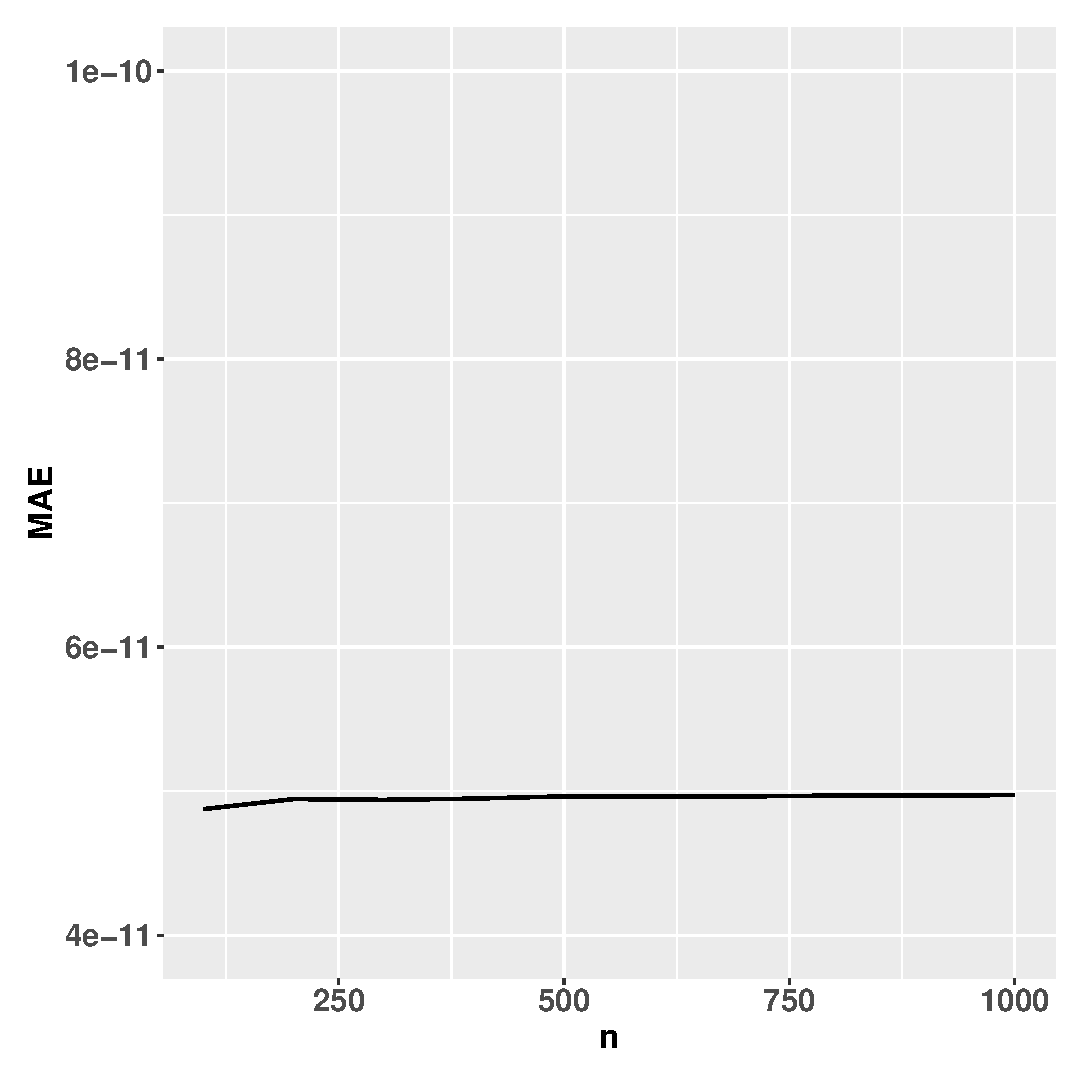
\includegraphics[width=1\textwidth]{figures/bino_mae.eps}
    \end{minipage}\hfill
    \begin{minipage}{0.45\textwidth}
        \centering
        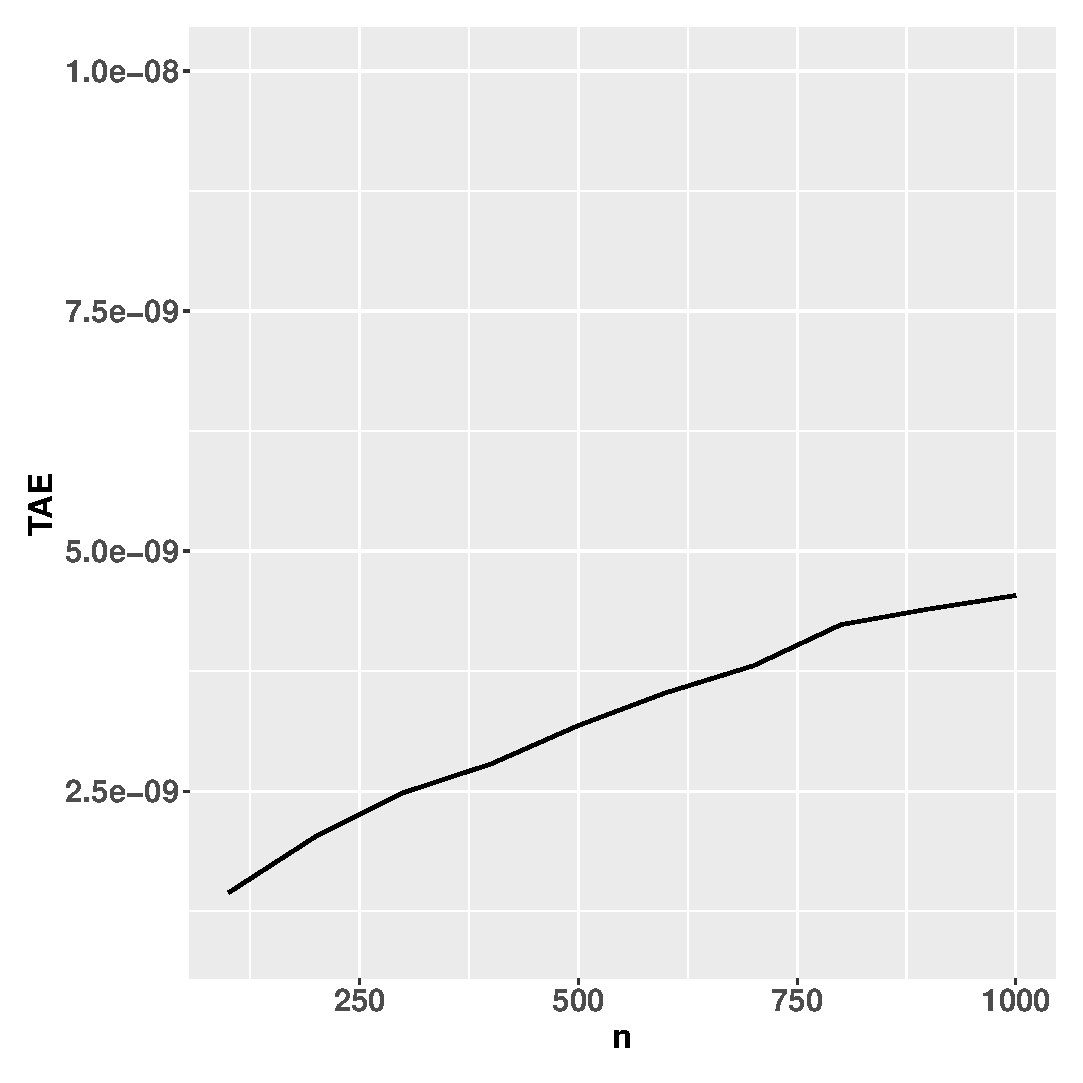
\includegraphics[width=1\textwidth]{figures/bino_tae.eps}
    \end{minipage}
    \caption{$\MAE$/$\TAE$ plots for the method $\dft$ using binomial distribution, $n$ increases up to 1000.}
    \label{fig:mae.tae.bino}
\end{figure}
To show that $\dft$ is able to calculate pmf exactly under the situation when $(n,m)$ is small enough to be calculated by enumeration, we randomly generate multiple $\Pmat$s from dimension $2 \times 2$ to $6 \times 4$ with smallest probability $0.007$ and largest probability $0.97$. The result shows that $\dft$ computes the pmfs exactly same as those computed by enumeration.
\begin{figure}
    \centering
    \begin{minipage}{0.45\textwidth}
        \centering
        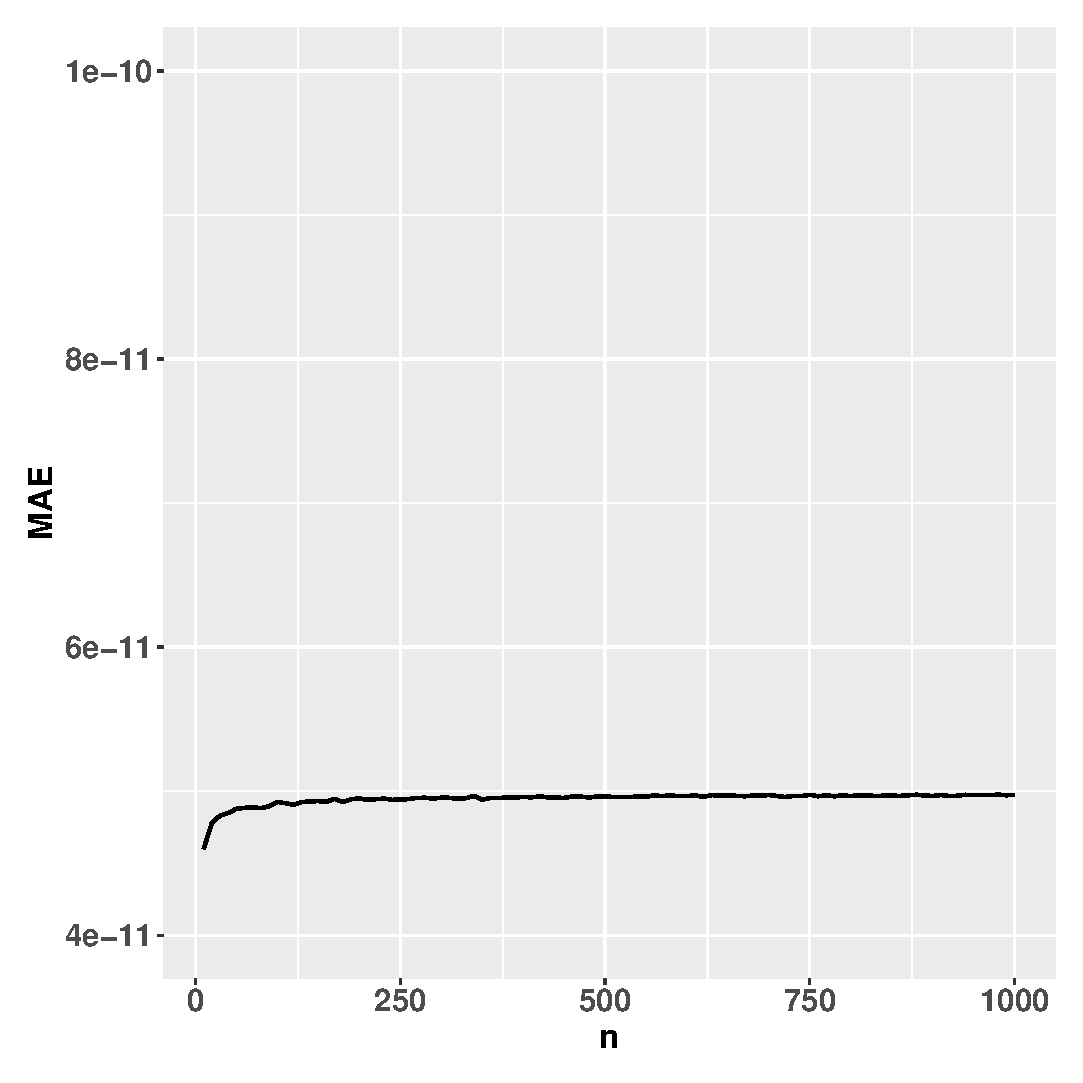
\includegraphics[width=1\textwidth]{figures/poi_mae.eps}
    \end{minipage}\hfill
    \begin{minipage}{0.45\textwidth}
        \centering
        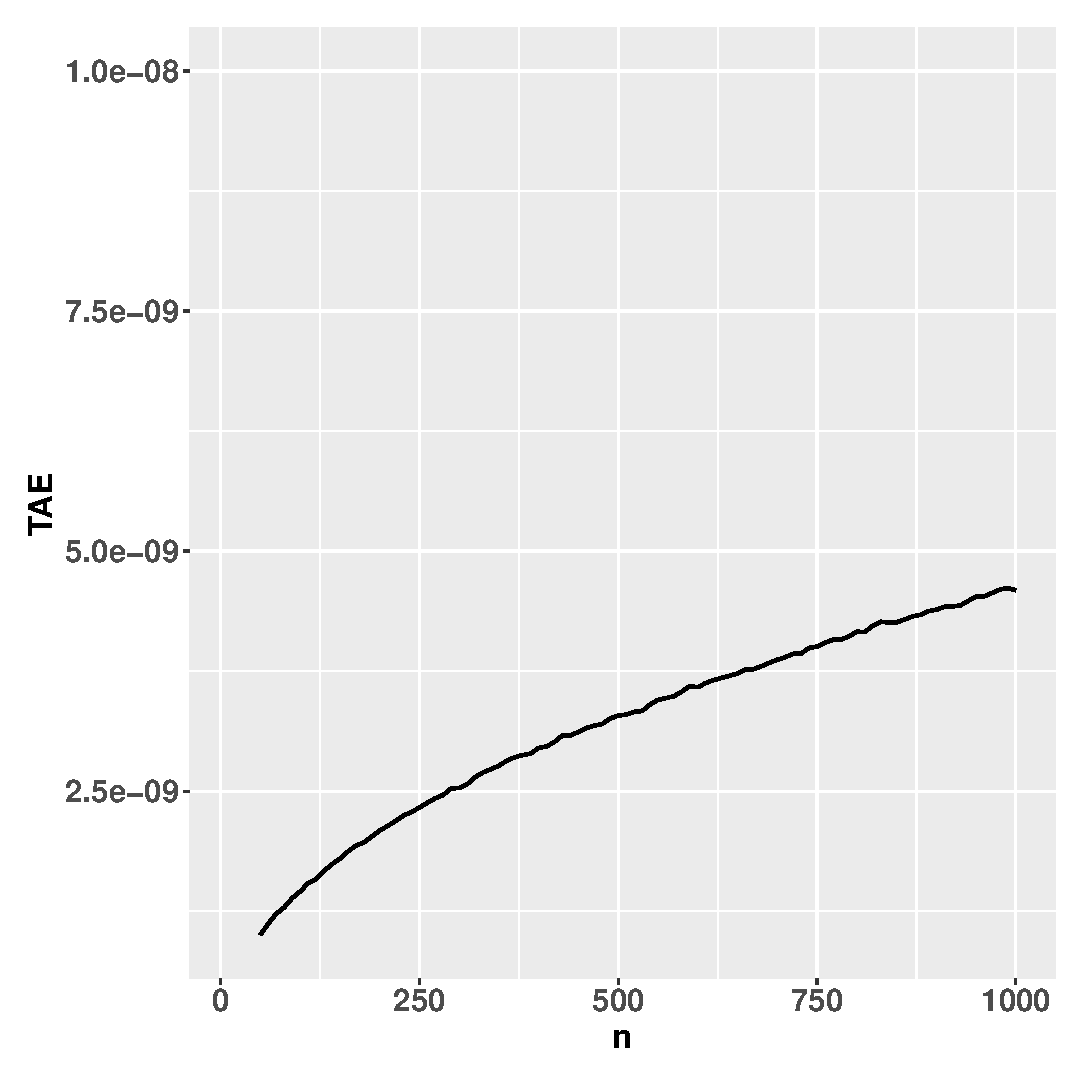
\includegraphics[width=1\textwidth]{figures/poi_tae.eps}
    \end{minipage}
    \caption{$\MAE$/$\TAE$ plots for the method $\dft$ using Poisson binomial distribution as $n$ increases up to 1000.}
    \label{fig:mae.tae.poi}
\end{figure}

Figure~\ref{fig:mae.tae.bino} and Figure~\ref{fig:mae.tae.poi} show the accuracy test result for the method $\dft$. In both plots, the $\MAE$ is smaller than $10^{-10}$. Also the total absolute error ($\TAE$) is well controlled and smaller than $10^{-9}$ generally. The error might come from the inside of the multi-dimensional discrete fast Fourier transformation algorithm. The multi-dimensional discrete fast Fourier transformation algorithms are usually less precise than the one dimensional discrete fast Fourier transformation algorithms.This is why when comparing with the result from \citeN{Hong2013}, our algorithm has larger $\MAE$ and $\TAE$. Figure~\ref{fig:mae.tae.poi} shows us similar results when the binomial is replaced by Poisson binomial, the patterns of $\MAE$ and $\TAE$ are almost looked same to the ones for binomial distribution. Therefore, changing distributions from special cases to general cases doesn't affect the accuracy of $\dft$. With respect to that, we can conclude that our $\dft$ algorithm is able to precisely compute pmf for $\PMD$ when $m$ and $n$ is large.



\subsection{Accuracy of Normal Approximation and Simulation Method}
%%%%%%%%%%%%%%%%%%%%%%%%%%%%%%%%%%%%%%%%%%%%%%%%%%%%%%%%%%%%%%%%%%%%%%%%%%%%%%%%%%%%%%%%%%%%%%%%%
Among the three computing algorithms we proposed, one of them is able to calculate the exact probability while the other two are approximation methods. Therefore, it is necessary to explore accuracy of the approximation methods under different circumstances. The accuracy metric for $\NA$ is $\MAE$. Probability mass points computed by $\dft$ are considered as true probabilities, denote it as $p_{\textrm{true}}$.
$\MAE$ for normal approximation is given by
\begin{equation*}
    \MAE = \max_{\xvec \in \chi}|p_{\NA}(\xvec)-p_{\textrm{true}}(\xvec)|.
\end{equation*}
Figure~\ref{fig:mae.na} illustrates the accuracy of the $\NA$ method. Specifically, in the plot we introduce a pattern called baseline to express the sparsity of $\PMD$ as $n$ and $m$ increase. The baseline is the $\MAE$ if we estimate all probability mass points at 0. Then for a given $\Pmat$, the value of baseline will be the max probability. Given $n$ and $m$,  randomly generate 5000 $\Pmat$s and use their average maximum probability as the value of baseline that showed in Figure~\ref{fig:mae.na} so that the effect of noise will be eliminated. It shows that the pattern of baseline is decreasing as $n$ increases, which describes the sparsity.
\begin{figure}%[h]
\begin{center}
	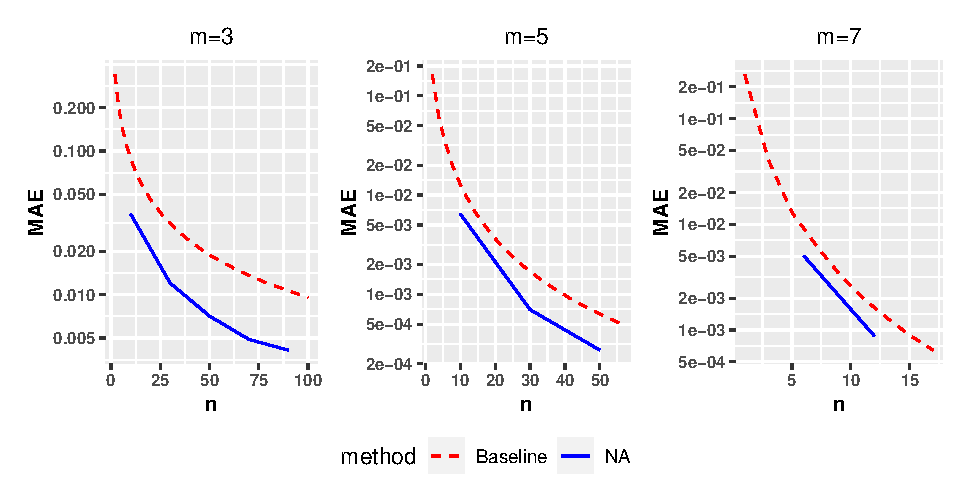
\includegraphics[width=0.95\textwidth]{figures/normal_mae.eps}
	\caption{$\MAE$ of $\NA$ compared with baseline when $m=3,5,7$}
	\label{fig:mae.na}
\end{center}
\end{figure}
From Figure~\ref{fig:accuracy.sim}, for given $m$, as $n$ increase the solid line which represents the method $\NA$ is always under the dashed baseline. The gap between the two lines grows wider as $n$ gets larger for fixed $m$, which indicates that $\NA$ gets more accurate when $n$ gets large despite of sparsity.

For $\SIM$ we only consider the probabilities at max, 0.95, and 0.90 quantiles due to computation limit of device. The accuracy metric for $\SIM$ is the absolute error. The absolute error metric is given by the absolute difference between the selected probability mass points (maximum, 0.95 and 0.90 quantiles) calculated by $\SIM$ and $\dft$.

For each $n$ from 1 to 75 and $m=3$, randomly generate 5000 $\Pmat$'s to exclude the noise effect. Then we calculate error metrics with respect to each methods. In this part, we mainly study the relation between accuracy and simulation $B$. The result is showed in Figure~\ref{fig:accuracy.sim}. In Figure~\ref{fig:accuracy.sim}, The solid lines represent the absolute error pattern of $B=10$, the dashed lines represents $B=10^5$ and the longdashed lines represent $B=10^7$. For each line, the pattern goes down as $n$ increases due to sparsity. Figure~\ref{fig:accuracy.sim} shows that $B=10$ is in general not precise while $B=10^7$ will have absolute error between $10^{-4}$ and $10^{-5}$, which is pretty accurate. Setting $B=10^5$ will have absolute error between $10^{-3}$ and $10^{-4}$.

Observe that the gap between lines reduces as $n$ increases possibly due to sparsity. The accuracy performance when $B$ is evidently better than when $B$ is small. We can tell from the plots that $B=10^7$ might be a good choice for user since it provide an accuracy error as small as $10^{-5}$.

\begin{figure}%[h]
\begin{center}
	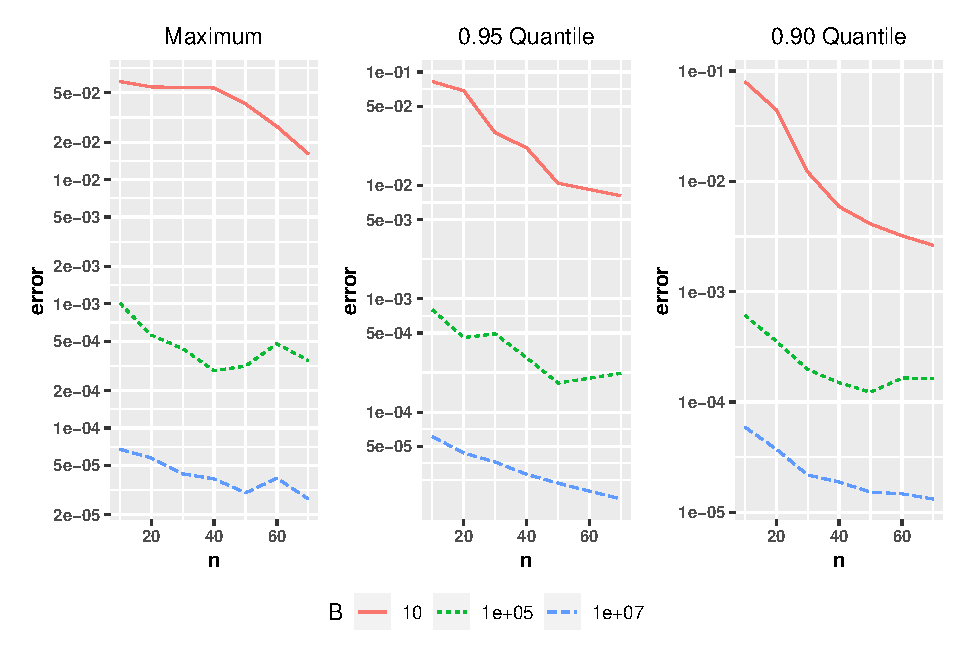
\includegraphics[width=0.95\textwidth]{figures/sim.eps}
	\caption{Absolute error of $\SIM$ method for $\PMD$ when $m=3$. The left plot compare the accuracy of different $B$ at maximum, the middle one and the right one do the same job at quantile 0.95 and 0.9 respectively. }
	\label{fig:accuracy.sim}
\end{center}
\end{figure}





%%%%%%%%%%%%%%%%%%%%%%%%%%%%%%%%%%%%%%%%%%%%%%%%%%%%%%%%%%%%%%%%%%%%%%%%%%%%%%%%%%%%%%%%%%%%%%%%%
\subsection{Time Efficiency of DFT-CF method}
As a method to compute the whole pmf, we need to consider $\dft$'s time efficiency especially when the dimension is large. Given a $\PMD$ with $\Pmat$ of $n \times m$ dimension, the method $\dft$ actually transforms a Fourier series of length $(n+1)^{m-1}$ since it takes every $x_j,j=1,\dots,m-1$ from 0 to $n$. The number of possible outcomes is $\binom{n+m-1}{m-1}$, so there will be a lot 0s in the pmf computed by $\dft$. The number $(n+1)^{m-1}$ increases drastically as $m$ gets large. When $m$ is small, the result is showed by Figure~\ref{fig:time.eff}. When $m$ is moderate ($8 \leq m \leq 20$) or larger, using $\dft$ can be problematic since $(n+1)^{m-1}$ will be enormous such that the device either takes too long to compute nor unable to compute due to exhausted usage of RAM. For example, let $m=8$ and $n=15$, the method $\dft$ will compute in total $16^7$ points, and it will be both time and memory consuming.

We use the same device as for accuracy study to test the time efficiency of $\dft$. Figure~\ref{fig:time.eff} plots the average computing time of 1000 randomly generated $\Pmat$'s using $\dft$. The scale of time is second(s). Figure~\ref{fig:time.eff} shows that when $m$ is small (less or equal to 4), it is good to use $\dft$ to calculate the entire pmf. As we can see from the plot that the computing time for $n=60, m=4$ is 16 seconds which is affordable. Even when $m=5$ and $n=40$ the time is around 100 seconds which is still acceptable. However, when $m=6$ or higher, increasing $n$ can make the computing time and memory cost unaffordable.


\begin{figure}%[h]
\begin{center}
	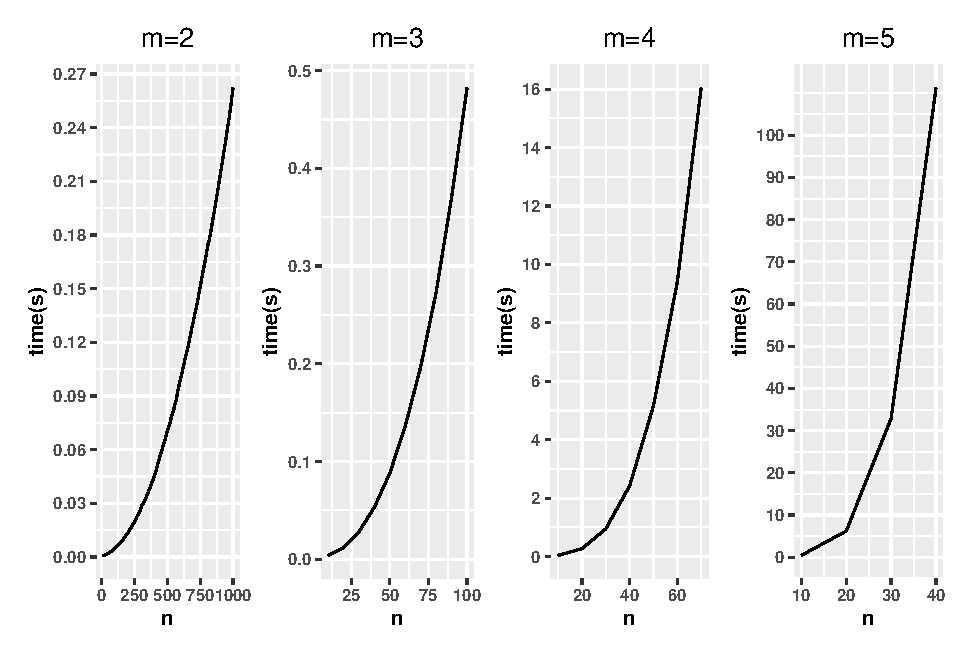
\includegraphics[width=0.95\textwidth]{figures/effi.eps}
	\caption{Time efficiency study of $\dft$.}
	\label{fig:time.eff}
\end{center}
\end{figure}


%%%%%%%%%%%%%%%%%%%%%%%%%%%%%%%%%%%%%%%%%%%%%%%%%%%%%%%%%%%%%%%%%%%%%%%%%%%%%%%%%%%%%%%%%%%%%%%%%
\subsection{Recommendations}
%%%%%%%%%%%%%%%%%%%%%%%%%%%%%%%%%%%%%%%%%%%%%%%%%%%%%%%%%%%%%%%%%%%%%%%%%%%%%%%%%%%%%%%%%%%%%%%%%
According to the results of accuracy and efficiency study. We hereby give out our recommendations of which method to choose under what circumstances. For small $m$ and moderate $n$, the $\dft$ can be used. Since the computing time is affordable and the method is an exact method that can compute the entire pmf automatically. On the other hand, when $m$ is moderate or large, this method can be very time consuming and will require huge RAM. Thus for moderate $m$ ($5 \leq m \leq 20$) and small $n$, we encourage users to use simulation method with $B$ around $10^6$ to calculate partial pmf of users' interests. By this way the accuracy will be maintained at a satisfied level and computing time will be affordable. For large $n$ including when $m$ is also large, the $\NA$ is recommended because the accuracy is backed up by central limit theory. In this case, if we only calculate partial pmf, computing time will not be a concern.

%%%%%%%%%%%%%%%%%%%%%%%%%%%%%%%%%%%%%%%%%%%%%%%%%%%%%%%%%%%%%%%%%%%%%%%%%%%%%%%%%%%%%%
\section{Applications}\label{sec:applications}
%%%%%%%%%%%%%%%%%%%%%%%%%%%%%%%%%%%%%%%%%%%%%%%%%%%%%%%%%%%%%%%%%%%%%%%%%%%%%%%%%%%%%%

In this section, we demonstrate applications of $\PMD$ in political science, ecological inference, and classification. In voting scenario, we suppose the number of voters and the number of candidates are both small for computational simplicity. We also assume the voting behavior of each voter is known. Then we can use $\PMD$ to model the voting process and calculate the probabilities for each candidates to win the election, and find out the most possible electoral result.

In ecological inference, we develop a logistic type model that uses $\PMD$ to compute likelihood for aggregated data. The raw dataset is the Predictive Maintenance Dataset Data Set \cite{Dua:2019} from UCI machine learning repository. In real world, aggregated data is usually formed based on historical information. In this paper, we form the aggregated dataset randomly for the purpose of illustrating the application of $\PMD$.

In classification, we illustrate an application of $\PMD$ in soft classification context using Electroluminescence (EL) image data. We train a CNN model using Relu activation function, and show that we can perform uncertainty quantification if we assume the confusion matrix follows $\PMD$.


\subsection{Calculation of Voting Probability}
In voting scenarios, people always pay attention to the election result. The most thing we usually care about is who will win the election and how many chances each candidate has to win the election. A Poisson multinomial distribution can fit the situation perfectly under some assumptions.

Suppose a election has $n$ voters and $m$ candidates, there will be $h = \binom{n+m-1}{m-1}$ possible outcomes denoted as $\xvec_r, r = 1, \dots, h$, respectively. Each $\xvec_r$ is a $m$ dimension vector that has three elements denoting the number of votes each candidate gets. Assume we know the $\Pmat$ based on prior polls, for example, we can always estimate the approval rate of each candidate in a certain constituency from the monthly polls or exit polls. Then we are able to compute the notional result.

To demonstrate that, suppose we have $n=10$ electoral voters and $m=3$ candidates with $\Pmat$ matrix that has means of column 1, 2 and 3 to be $0.3631,0.3405$ and $0.2964$, the first five rows are as following,
\begin{equation*}
\begin{pmatrix}
0.071 & 0.589 & 0.340\\
0.365 & 0.195 & 0.440\\
0.445 & 0.505 & 0.050\\
0.353 & 0.382 & 0.265\\
0.620 & 0.111 & 0.269
    \end{pmatrix}
\end{equation*}
To compute the probability of each candidate winning the election, just need to introduce constraints. For instance, under the constraint $\chi_1 = \left\{\text{the first element is the largest one}\right\} = \left\{x_1>x_2, x_1>x_3; x_1, x_2,x_3 \in \left\{0,\dots,10\right\}\right\}$, we are able to compute the winning rate of the first candidate is
\begin{equation*}
\Pr(\text{the 1st candidate wins}) = \sum_{\xvec \in \chi_{1}} p(\xvec) = 0.3429
\end{equation*}
Similarly, the probabilities for the second candidate and the third candidate to win are $0.2745$ and $0.2001$. Additionally, the most possible result is $\xvec=(4,3,3)'$, which has probability 0.08546.




%%%%%%%%%%%%%%%%%%%%%%%%%%%%%%%%%%%%%%%%%%%%%%%%%%%%%%%%%%%%%%%%%%%%%%%%%%%%%%%%%%%%%%
\subsection{Statistical Inference for Aggregated Data}\label{sec:model.est.inf}	
First introduce the logistic type model to fit a given aggregated dataset with selected covariates and a categorical response variable that has $m$ categories.

By dividing the rows of our data into $h$ groups via some given criterion, the group size of each group is $n_i,i=1,\dots,h$. Each $n_i$ are positive integer but not necessarily equal to each other. Let the counts for the aggregated response variable of the $i$th group be
$\xvec_i = (x_{i1}, \dots,x_{im})'$, where $m$ is the category number. Denote $\Gmat_i$ to be the covariate matrix of the $i$th group, then $\Gmat_i = (\onevec', \gvec_{i 1}',\dots,\gvec_{i n_i}')'$ is a $n_i \times (v+1)$ matrix with first column being $\onevec$, where $v$ is the number of covariates. Let $\Pmat_i = (p_{ijk})$ be the SPM for the $i$th group, $i = 1, \dots, h$, $j = 1,\dots ,n_i$ and $k = 1,\dots, m$. Let the probability of getting $\xvec_i$ for the $i$th group be $p(\xvec_i)$. The total log-likelihood for all groups can be computed as
\begin{equation*}
\loglik(\betavec) = \sum_{i=1}^{h}\loglik_i(\betavec) = \sum_{i=1}^{h}\log[p(\xvec_i)],
\end{equation*}
where $p(\xvec_i)$ can be computed via $\PMD$ with SPM $\Pmat_i$. Set category $m$ as baseline and use softmax function to form the $\Pmat_i$ for each group through parameter $\betavec = (\betavec_1', \dots, \betavec_{m-1}')'$ as
\begin{align*}
    p_{i j k} = \frac{\exp{\left(\gvec_{ij}' \betavec_{k}\right)}}{1 + \sum_{k=1}^{m-1}\exp{\left( \gvec_{ij}' \betavec_{k} \right)}},
    \quad k \neq m, \quad \text{and } \quad
    p_{i j m} = \frac{1}{1 + \sum_{k=1}^{m-1}\exp{\left( \gvec_{ij}' \betavec_{k} \right)}}.
\end{align*}
%The likelihood will become
%\begin{equation*}
%\loglik (\betavec) = \sum_{i=1}^{h}\loglik_i (\betavec)= \sum_{i=1}^{h}\log[ p(\xvec_i)].
%\end{equation*}
Then we are able to estimate our parameters on the direction of minimizing total log-likelihood and finally get our estimate $\wh{\Pmat}_i$.

In the rest of this part, we apply the model to the
AI4I 2020 Predictive Maintenance Dataset ``ai4i"  \cite{Dua:2019}. The dataset ``ai4i" is a synthetic machine failure dataset that reflects real predictive maintenance data encountered in industry. The data consists of 10000 products (rows) and 14 features (columns) including Product type, Air temperature, Process temperature, Rotational speed and others.

For demonstration purpose, here we only use the first 1000 rows and Product type as response variable, Air temperature and Process temperature as covariates. The feature Product type is categorical and has three levels, ``M", ``L", ``H", we denote them as category 1, 2, 3 for simplicity. The number of products that fall in category 1, 2, and 3 are 285, 601, and 114. The other two features are continuous.


We randomly divide the dataset into 100 groups, the smallest group has size of three rows and the largest one has 18 rows. Note that readers can use other criterion to divide the dataset by their own. Notice the covariate number is three including intercept and the response has three categories, thus the dimension of our parameter matrix $\betavec$ will be $3 \times 2$ if we set category 3 as baseline.

The estimates of the parameters are
\begin{equation*}
\wh{\betavec} =
\begin{pmatrix}
 1.07484986 & 2.2820922 \\
 1.62342045 & 1.9108976 \\
 -0.06277732 &-0.8455964\\
\end{pmatrix}
\end{equation*}
The corresponding $\wh{\Pmat}_1$ and $\wh{\Pmat}_5$ for group 1 and group 5 are
\begin{equation*}
    \wh{\Pmat}_1 = \begin{pmatrix}

 0.11914 & 0.63310 & 0.24776\\
 0.12326 & 0.57268 & 0.30406\\
 0.14809 & 0.47560 & 0.37631\\
 0.14504 & 0.56971 & 0.28525\\
 0.12451 & 0.54095 & 0.33454\\
 0.04170 & 0.55944 & 0.39886\\
 0.03559 & 0.53568 & 0.42873\\
 0.04890 & 0.54668 & 0.40442
    \end{pmatrix}, \quad
    \wh{\Pmat}_5= \begin{pmatrix}
 0.15604 & 0.70766 & 0.13630\\
 0.14469 & 0.73976 & 0.11555\\
 0.11246 & 0.67372 & 0.21382\\
 0.12036 & 0.64885 & 0.23079\\
 0.11263 & 0.61304 & 0.27433\\
 0.11563 & 0.55029 & 0.33408\\
 0.11774 & 0.61672 & 0.26554\\
 0.15071 & 0.52510 & 0.32419\\
 0.13878 & 0.56645 & 0.29477\\
 0.08194 & 0.54561 & 0.37245\\
 0.06307 & 0.58191 & 0.35502
    \end{pmatrix}
\end{equation*}
For group 1 and 5, $\xvec_1 = (1,5,2)'$ and $\xvec_5 = (2,6,3)'$, so $p(\xvec_1) = 0.070$, $p(\xvec_5) = 0.067$.
%%%%%%%%%%%%%%%%%%%%%%%%%%%%%%%%%%%%%%%%%%%%%%%%%%%%%%%%%%%%%%%%%%%%%%%%%%%%%%%%%%%%%%

%%%%%%%%%%%%%%%%%%%%%%%%%%%%%%%%%%%%%%%%%%%%%%%%%%%%%%%%%%%%%%%%%%%%%%%%%%%%%%%%%%%%%%
\subsection{Uncertainty Quantification in Classification}
In machine learning classification problem with multiple labels, for each unit in the test set, the probability of the unit belongs to each class is computed. Usually, the predicted class is assigned as the highest probability. Using the soft classifiers, the unit class is randomly assigned according to the predicted probabilities, leading to randomness in the confusion matrix. The PMD can be used to characterize the distribution of the counts in the confusion matrix.

In this section, we consider an Electroluminescence (EL) image classification example to illustrate the usage of PMD in machine learning classification problems. In the photovoltaic (PV) reliability study, the EL image is an important data type that reveal information about the PV health status. Because disconnected parts do not irradiate, the darker areas in EL images indicate defective cells. The EL imaging provide visual inspection of solar panels and is a non-destructive technology for failure analysis of PV modules \shortcite{Deitsch2019}.

The work of \shortciteN{Deitsch2019}, \shortciteN{Buerhop2018}, and \shortciteN{Deitsch2021} provide a public dataset of solar cells extracted from high resolution EI images of PV modules (\url{https://github.com/zae-bayern/elpv-dataset}). In total there are 2624 images. All images are preprocessed with respect to size and are eliminated distortion induced by the camera lens used to capture the EL images. Each image is manually labeled  with its degree of defectiveness. The degree of defectiveness is determined by two questions. The first is how do evaluators think the status of the solar cells, functional or defective; the second is how they are confident about their assessments. In total there are four labels as shown in Table \ref{tbl:el.label} and we marked them as Class A-D.

\begin{table}%[h!]
\caption{Partitioning of solar cells into functional and defective, with an additional self-assessment on the rater's confidence after visual inspection. Non-confident decisions obtain a weight lower than 100\% for the evaluation of the classifier performance.}\label{tbl:el.label}
\begin{center}	
\begin{tabular}{c|c|c|c|c}
		\hline
		\hline
		Condition  & Confident  &  Label $p$ & Weight $w$ & Class \\
		\hline
		\multirow{2}{*}{functional} & Yes & functional & 0\% & A\\
		& No& defective  & 33\% & B\\
		\hline
		\multirow{2}{*}{defective} & No & defective & 67\% & C\\
		& Yes & defective & 100\%  &D\\
		\hline
		\hline
	\end{tabular}
\end{center}
\end{table}
%According to the probability how likely the product is defective, we assign four labels to sollar cells, 0\%, 33.33\%, 66.66\%, 100\%.

We split our data to training data (80\%) and test data (20\%), then train a CNN \cite{DBLP:journals/corr/LongSD14} model on the training set. In CNN model, we use Relu activation function and set the kernel size $3 \times 3$ and stride $1 \times 1$. For each image in the testing set, the model provides a probability that the prediction belongs to each class. Table~\ref{tbl:elpmat} provides a subset of the CNN model output. For true class for the first sample in Table~\ref{tbl:elpmat} is A. If we predict the class of the first sample using the highest probability, then the prediction is A and there's no randomness. If we allow the model to make predictions based on the probability vector as shown in the first row then there are randomness in the confusion matrix. We can consider the confusion matrix to follow a PMD distribution then we can quantify the uncertainty in confusion matrix using PMD.

Figure~\ref{fig:confusion.hist} shows the marginal probability of each cell. For example, in the first row first column panel cell in Figure~\ref{fig:confusion.hist}, we know the possible counts that the model correctly predict class A as well as the corresponding probability. In this way, we have a uncertainty quantification in the confusion matrix.


\begin{table}%[ht]
\begin{center}
\caption{An example of the probability vectors of a subset in testing set from the trained CNN model.}\label{tbl:elpmat}
\begin{tabular}{rrrrr}
  \hline\hline
 & A & B & C & D \\
  \hline
1 & 0.9230 & 0.0366 & 0.0107 & 0.0297 \\
  2 & 0.0736 & 0.0802 & 0.0513 & 0.7950 \\
  3 & 0.0000 & 0.0016 & 0.0006 & 0.9978 \\
  4 & 0.9170 & 0.0537 & 0.0062 & 0.0231 \\
  5 & 0.9579 & 0.0239 & 0.0070 & 0.0112 \\
  6 & 0.8991 & 0.0347 & 0.0132 & 0.0530 \\
   \hline\hline
\end{tabular}
\end{center}
\end{table}


\begin{figure}
\begin{center}
	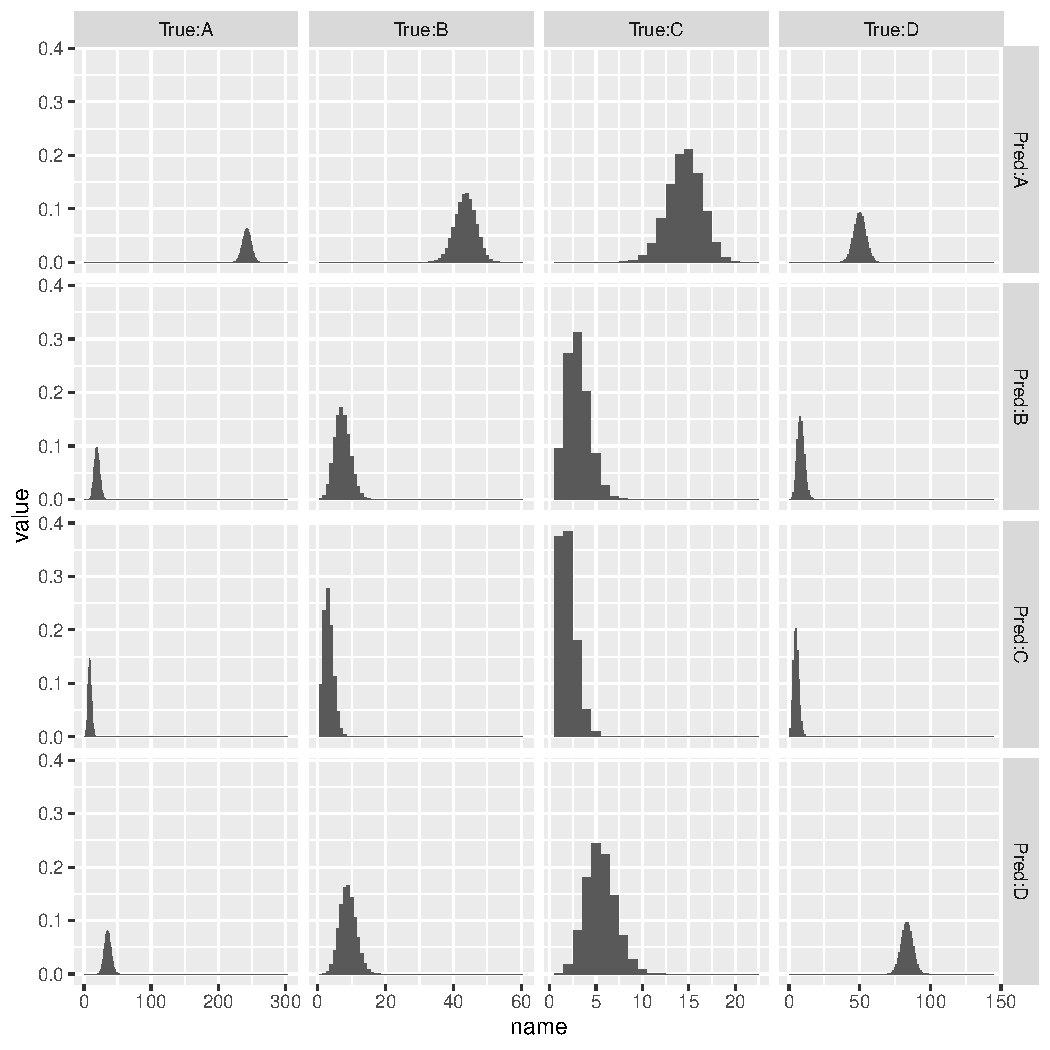
\includegraphics[width=0.9\textwidth]{figures/Confusionbar.pdf}
	\caption{The barplot shows the confusion matrix prediction. For each panel cell, the plot shows the corresponding prediction counts fall in this cell as well as their probability. We also present the mean and 95\% naive prediction interval.}
	\label{fig:confusion.hist}
\end{center}
\end{figure}


%%%%%%%%%%%%%%%%%%%%%%%%%%%%%%%%%%%%
\section{Illustrations of the R Package}\label{sec:rpackage}
%%%%%%%%%%%%%%%%%%%%%%%%%%%%%%%%%%%%%%%%%%%%%%%%%%%%%%%%%%%%%%%%%%%%%%%%%%%%%%%%%%%%%%%%%%%%%%%%%
We develop an R package named $\textrm{PoissonMultinomial}$ that computes probability density function for $\PMD$ with corresponding $\Pmat$ using the methods described by this paper. The package includes all methods we develop in this paper, and are able to compute the pmf, cdf of a given $\PMD$ as well as generating $\PMD$ random samples.

There are three major functions in the package. $\code{dpmd}$ is a function to compute pmf, $\code{ppmd}$ is for cdf and one can use $\code{rpmd}$ to generate $\PMD$ random samples. User has to specify $\Pmat$ so that a $\PMD$ can be determined. With unspecified $\xvec$, $\code{dpmd}( )$ will automatically calculate the whole pmf and the output will be a multi-dimensional array. If user inputs $\xvec$, the output of $\code{dpmd}( )$ will be partial pmf chosen by $\xvec$. User can also select all methods we list in this paper to compute the pmf or cdf. Notice only $\dft$ can automatically compute the whole pmf and it is the most efficient way for this job as well. The function $\code{ppmd}$ uses same method as $\code{dpmd}$ to compute the probability $\Pr(\Xvec \leq \xvec)$ and the function $\code{rpmd}$ generates random samples from $\PMD$.  Examples of using $\code{dpmd}$ is following,

First, $\code{pp}$ is an input matrix that specifies a $\PMD$. It looks as
\begin{verbatim}
  > pp=matrix(c(0.1, 0.1, 0.1, 0.7,
              0.1, 0.3, 0.3, 0.3,
              0.5, 0.2, 0.1, 0.2),
              byrow=T, ncol=4, nrow=3)
\end{verbatim}
%$$
%\begin{pmatrix}
%0.1 & 0.1 & 0.1& 0.7\\
%0.1 &0.3 & 0.3 & 0.3\\
%0.5  &0.2 & 0.1 & 0.2
%\end{pmatrix}
%$$
and $\xvec=(0,0,1,2)'$. Then the codes of using $\code{dpmd}$ to calculate pmf, is given as following
\begin{verbatim}
  > dpmd(pmat = pp)
  > dpmd(pmat = pp, xmat = x)
  > dpmd(pmat = pp, xmat = x, method = "NA" )
  > dpmd(pmat = pp, method = "SIM", B = 1e3)
  > dpmd(pmat = pp, xmat = x, method = "SIM", B = 1e3)
\end{verbatim}

The first line computes the whole pmf, the second one computes partial pmf of given $\xvec$, the rest of the codes just do the similar job using $\NA$ and $\SIM$.

We shall demonstrate the one to one map between the output and the pmf of an $n \times m$ $\PMD$. First we have a location indicator vector $v = (v_1, \dots, v_{m-1})'$ and an $\xvec=(x_1,\dots,x_m)'$, let $v_j-1 = x_j, j =1,\dots,m-1$ then the array element with location $v$ has the value of $\Pr(X=\xvec)$. We further illustrate this map via the $\Pmat$ given above.

The $\Pmat$ is $3 \times 4$ so the output of $\code{dpmd}$ is a $4 \times 4 \times 4$ dimensional array listed in the following matrices~\ref{verba:1}. Since the input $\code{pp}$ is dimension $3 \times 4$, the output is an $4 \times 4 \times 4$ array. First consider the element of row 3 column 2 in the first matrix of the matrices~\ref{verba:1}. Then the first two elements of $v$ is 3 and 2. The third element depends on the comma number on the top of each figure. On the top of the first matrix there are two commas followed by 1, thus the third element of $v$ is 1. Now we have constructed $v = (3,2,1)$, then we minus 1 on each element we get $\xvec=(2,1,0)'$ which is the corresponding probability mass point. So far we can get the element that has location indicated by $v=(3,2,1)$ is 0.022 and we have $\Pr(X=(2,1,0)')=0.022$.

In the other direction, if we want to know the probability of $\Xvec=\xvec$, where $\xvec=(0,3,0)'$. we need to construct its corresponding $v$, which can be computed by plus 1 to each element in $\xvec$ so that we get $v=(1,4,1)$. The $v$ we just constructed indicates a location of (1,4,1) of our array. That location is the first row, 4th column in the $\text{, , 1}$ placement of the $\code{res}$, which has value 0.006.

\begin{verbatim}
 > res <- dpmd(pmat=pp)
 > res
  , , 1                              , , 2
        [,1]  [,2]  [,3]  [,4]             [,1]  [,2]  [,3] [,4]
  [1,] 0.042 0.090 0.054 0.006       [1,] 0.069 0.084 0.015    0
  [2,] 0.125 0.148 0.023 0.000       [2,] 0.138 0.042 0.000    0
  [3,] 0.052 0.022 0.000 0.000       [3,] 0.021 0.000 0.000    0
  [4,] 0.005 0.000 0.000 0.000       [4,] 0.000 0.000 0.000    0
  , , 3                              , , 4
        [,1]  [,2] [,3] [,4]               [,1] [,2] [,3] [,4]
  [1,] 0.030 0.012    0    0         [1,] 0.003    0    0    0
  [2,] 0.019 0.000    0    0         [2,] 0.000    0    0    0
  [3,] 0.000 0.000    0    0         [3,] 0.000    0    0    0
  [4,] 0.000 0.000    0    0         [4,] 0.000    0    0    0
\end{verbatim}
\label{verba:1}

%\begin{figure}
%  \begin{subfigure}{8cm}
%    \centering
%    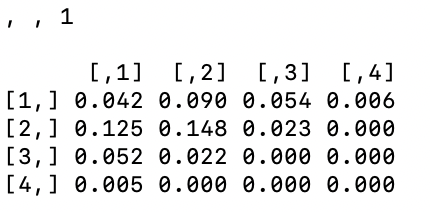
\includegraphics[width=7cm]{figures/1.png}
%    \caption{ }
%  \end{subfigure}
%  \begin{subfigure}{9cm}
%    \centering
%    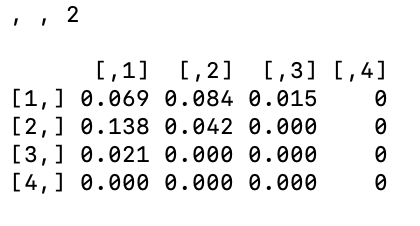
\includegraphics[width=7cm]{figures/2.png}
%    \caption{ }
%  \end{subfigure}
%  \begin{subfigure}{8cm}
%    \centering
%    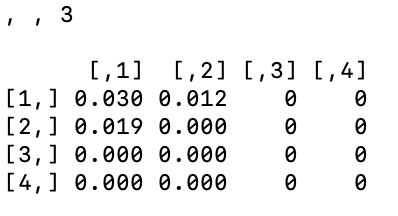
\includegraphics[width=7cm]{figures/3.png}
%    \caption{ }
%  \end{subfigure}
%  \begin{subfigure}{9cm}
%    \centering
%    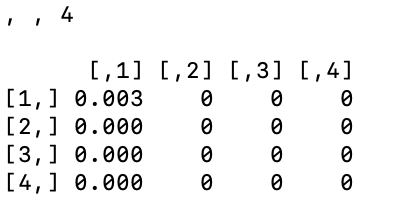
\includegraphics[width=7cm]{figures/4.png}
%    \caption{ }
%  \end{subfigure}
%\end{figure}



%%%%%%%%%%%%%%%%%%%%%%%%%%%%%%%%%%%%%%%%%%%%%%%%%%%%%%%%%%%%%%%%%%%%%%%%%%%%%%%%%%%%%%%%%%%%%%%%%
\section{Conclusions and Areas for Future Research}\label{sec:conclusion}
%%%%%%%%%%%%%%%%%%%%%%%%%%%%%%%%%%%%%%%%%%%%%%%%%%%%%%%%%%%%%%%%%%%%%%%%%%%%%%%%%%%%%%%%%%%%%%%%%

We develop three methods that can be useful for computing the pmf of the PMD, which is challenging to compute but useful in many application scenarios. We include the three methods we designed in an R package. Among the methods, $\dft$ is an exact method, $\SIM$ is a simulation method and $\NA$ is a method using approximation theories. The accuracy and efficiency of the methods are guaranteed under given circumstances. We recommend users to use $\dft$ when $m$ is small, use $\SIM$ when $m$ is moderate and $n$ is small, use $\NA$ when $n$ is large.


However, there are still some fields remain to be explored. The computing speed of $\dft$ can be improved using more efficient Fourier transformation algorithms or we could find a way to calculate only the $\binom{n+m-1}{m-1}$ possible outcomes rather than $(n+1)^{m-1}$ probability mass points which contains a large amount of points with values equal to 0. $\SIM$ method is still time consuming although it can compute some cases that $\dft$ are unable to, once we develop more efficient exact algorithms, $\SIM$ could be replaced. Until now, we are still unable to compute the pmf of $\PMD$ when $m$ is large due to the computational limit of machines, this area remains to be disclosed.

%%%%%%%%%%%%%%%%%%%%%%%%%%%%%%%%%%%%%%%%%%%%%%%%%%%%%%%%%%%%%%%%%%%%%%%%%%%%%%%%%%%%%%%%%%%%%%%%%%%%%%%%%%%%%%%%%%%%

%\section*{Acknowledgments}
%%%%%%%%%%%%%%%%%%%%%%%%%%%%%%%%%%%%%%%%%%%%%%%%%%%%%%%%%%%%%%%%%%%%%%%%%%%%%%%%%%%%%%%%%%%%%%%%%%%%%%%%%%%%%%%%%

%\bibliographystyle{apacite}


\bibliographystyle{chicago}
%\bibliography{refs.BIB}	
\bibliography{refs}	

\end{document}

%%%%%%%%%%%%%%%%%%%%%%%%%%%%%%%%%%%%%%%%%%%%%%%%%%%%%%%%%%%%%%%%%%%%%%%%%%%%%%%%%%%%%%%%%%%%%%%%%%%%%%%%%%%%%%%%%%%%%%%%%%%%%%%%%%%%%%%

